%
% Reproducibility manuscript: describe results from relative
% alchemical free energy simulation done with various MD packages.
%
% arara: make
% arara: pdflatex
% arara: bibtex
% arara: pdflatex
% arara: pdflatex
% arara: clean: {files: [reprod.aux, reprod.bbl, reprod.blg, reprod.log,
%acs-reprod.bib, reprod.lod, reprod.fls]}
%

\documentclass[journal=jctcce,manuscript=article]{achemso}

\usepackage[T1]{fontenc}
\usepackage{graphicx}
\usepackage{amsmath,amssymb,mathrsfs}
\usepackage{xr}
\usepackage{booktabs}
\usepackage{multirow}
\usepackage{rotating}
\usepackage{siunitx}
\usepackage{nameref}
\usepackage{easy-todo}
\usepackage{arydshln}
\usepackage{footref}


\externaldocument[S-]{SI}

\sisetup{
  separate-uncertainty = true
}

\newcommand{\progname}[1]{\texttt{#1}}
\newcommand{\inpopt}[1]{\texttt{#1}}

\renewcommand{\vec}[1]{\mathbf{#1}}
\renewcommand{\footnoterule}{}

\renewcommand\thetable{{\bf \arabic{table}}}
\renewcommand{\tablename}{{\bf Table}}

\renewcommand\thefigure{{\bf \arabic{figure}}}
\renewcommand{\figurename}{{\bf Figure}}

\title{Reproducibility of Free Energy Calculations Across Different Molecular Simulation Software}
%\title{\color{red}Reproducibility Limit of Free Energy Perturbation (FEP) Calculations}
%\title{Comparison of Free Energy Calculations Between Different Molecular Simulation Software}
%\title{Are FEP Calculations Reproducible?}

\author{Hannes H. Loeffler}
\affiliation[Scientific Computing Department, STFC]{Science \&
  Technology Facilities Council, Daresbury, Warrington, WA4 4AD,
  United Kingdom}
\email{Hannes.Loeffler@stfc.ac.uk} \phone{+44 1925 603367}

\author{Stefano Bosisio}
\affiliation[University of Edinburgh]{EaStCHEM School of Chemistry,
  University of Edinburgh, David Brewster Road, Edinburgh EH9 3FJ, UK}

\author{Guilherme Duarte Ramos Matos}
\affiliation[University of California, Irvine]{Department of
  Chemistry, University of California, Irvine}

\author{Donghyuk Suh}
\affiliation[University of Chicago]{University of Chicago}

\author{Julien Michel}
\affiliation[University of Edinburgh]{EaStCHEM School of Chemistry,
  University of Edinburgh, David Brewster Road, Edinburgh EH9 3FJ, UK}

\author{David L. Mobley}
\affiliation[University of California, Irvine]{Departments of
  Pharmaceutical Sciences and Chemistry, University of California,
  Irvine}

\author{Benoit Roux}
\affiliation[University of Chicago]{University of Chicago}


\keywords{Free Energy, Hydration, Alchemical, Reproducibility, Automation}

\begin{document}

\begin{abstract}
  Alchemical free energy calculations are an increasingly
  important modern simulation technique.  Contemporary molecular
  simulation software such as AMBER, CHARMM, GROMACS and SOMD include
  support for the method.  Implementation details vary among those
  codes but users expect reliability and reproducibility, i.e.\ for a
  given molecular model and set of forcefield parameters, comparable
  free energy should be obtained within statistical bounds regardless
  of the code used.  \emph{Relative} alchemical free energy (RAFE)
  simulation is increasingly used to support molecule discovery
  projects, yet the reproducibility of the methodology has been less
  well tested than its absolute counterpart.  Here we present
  RAFE calculations of hydration free energies for a set
  of small organic molecules and demonstrate that free energies can be
  reproduced to within about \SI{0.2}{kcal/mol} with aforementioned
  codes.  Absolute alchemical free energy simulations have been
  carried out as a reference.  Achieving this level of reproducibility
  requires considerable attention to detail and package--specific
  simulation protocols, and no universally applicable protocol
  emerges. The  benchmarks and protocols reported here should be
  useful for the community to validate new and future versions of
  software for free energy calculations.
\end{abstract}

\begin{tocentry}
  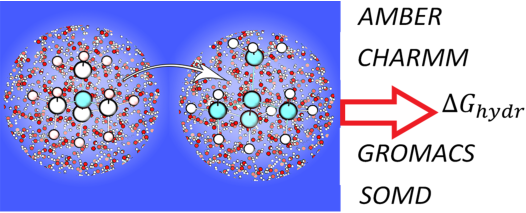
\includegraphics[scale=1.0]{figures/final_toc.pdf}
\end{tocentry}

\section{Introduction}
\label{sec:intro}

The free energy is a fundamental function of thermodynamics as it explains
how processes in nature evolve.  The equilibrium balance of products and reactants in a hypothetical chemical reaction can be immediately determined
from the knowledge of the free energy difference of reactants and
products and their concentrations.  The free energy landscape of a given
system, however, can be very complicated and rugged with barriers which impose
limits on how fast the process can take place.  It is therefore of
little surprise that the determination of free energy changes is of
utmost importance in the natural sciences, e.g.\ for binding and
molecular association, solvation and solubility, protein folding and
stability, partition and transfer, and design and improvement of force
fields.

The calculation of free energies via molecular
simulations~\cite{hansen_practical_2014, doi:10.1021/jp102971x,
  Gallicchio201127, doi:10.1080/08927022.2015.1132317,
  doi:10.1146/annurev.matsci.32.111901.153708} has been particularly
attractive as it promises to circumvent certain limitations of experimental
approaches. Specifically, processes can be understood at the atomic level and there is the potential that computational techniques can be
more cost and time effective, especially if they can predict the properties of new molecules before their synthesis.
Thus, a multitude of methods have been devised
 to make reversible work estimates accessible through
computation~\cite{hansen_practical_2014,
  doi:10.1021/jp102971x, Gallicchio201127,
  doi:10.1080/08927022.2015.1132317,
  doi:10.1146/annurev.matsci.32.111901.153708}.  However, the
reliability of estimates is still very much a matter of
concern~\cite{doi:10.1021/jp102971x, doi:10.1021/acs.jctc.5b00179}.

Here we are interested in \emph{alchemical} free energy methods because they
are firmly rooted in statistical thermodynamics and should give asymptotically
correct free energy estimates, i.e.\ they are correct for a given potential
energy function in the limit of sufficient simulation
time~\cite{Beveridge-citeulike:3789890, straatsma:92, doi:10.1021/cr00023a004,
hansen_practical_2014}.
The method has been applied in various forms for
several decades now since the early days of computer
simulation~\cite{doi:10.1063/1.1671118, bennett_efficient_1976,
doi:10.1063/1.432264, FS9821700055,  Tembe1984281, doi:10.1063/1.449208}.
The method is also increasingly referred as free energy perturbation (FEP)  in the literature, even though different techniques may have actually been used to estimate free energy changes.
The method has gained renewed attention in recent years --- concomitant with
improvements in computer hardware design --- within the traditional equilibrium
framework~\cite{GILSON19971047, doi:10.1021/jp0217839, deng_computations_2009}
and also increasingly in combination with non-equilibrium
techniques~\cite{ytreberg_comparison_2006, JCC:JCC23804,
  doi:10.1021/ct500964e}.  The name ``alchemical'' comes from the nonphysical
intermediates that often need to be created to obtain reliable estimates of
free energy differences between physical end states, and because parts or
all of a molecule may effectively appear or disappear in a transformation.  In the
context of force field methods the transformation takes place in parameter
space, i.e.\ the various force field parameters are varied by scaling.  This
can be a particularly efficient approach compared to methods involving physical transition pathways or order parameters, as it does not require sampling of
diffusive motions, avoids crossing prohibitively large energy barriers if
transition pathways are not well chosen, and is easier to automate.

Alchemical free energy simulations rely on the concept of thermodynamic
cycles~\cite{Tembe1984281}.
As the free energy is a state function, the sum of free energy changes
computed around any closed cycle must be zero.  This also implies
that the reversible work can be computed along
conveniently chosen legs of the cycle, even if the cycle is artificial.  For example, in
Fig.~\ref{fig:thermocycle} the relative free energy of hydration can
be computed along the vertical legs, that is, following the physical
process of moving a molecule from the gas phase to the liquid phase,
or along the horizontal legs in a non-physical but computationally more
efficient alchemical calculation.

\begin{figure}[ht]
  
\includegraphics[scale=1.0]{figures/thermocycle.pdf}
  \caption{The thermodynamic cycle to compute the relative free energy
    of hydration
    $\Delta\Delta G_{\mathrm{hydr}}=\Delta G_{\mathrm{sol}}-\Delta
    G_{\mathrm{vac}}=\Delta G'' - \Delta G'$.  The example is for the
    ethanol $\leftrightarrow$ methanol transformation.  A blue background indicates water and a white background indicates gas phase. Alchemical
    simulations are performed along the non-physical horizontal
    legs while vertical legs illustrate the physical process of moving a
    molecule from the vacuum to the solution.  The latter is also accessible
    through absolute alchemical free energy simulation, see e.g.\
    Ref.~\citenum{doi:10.1021/acs.jced.7b00104}.}
  \label{fig:thermocycle}
\end{figure}

Absolute (standard) alchemical free energy calculation has been of
particular interest for many years~\cite{GILSON19971047,
  doi:10.1021/jp0217839, deng_computations_2009, ytreberg_comparison_2006, doi:10.1021/ct500964e, jorgensen1988efficient}.  \emph{Absolute}
here really means that the equilibrium constant of a physical
reaction, e.g.\ binding and dissociation, can be calculated directly
by completely decoupling or annihilating a whole molecule from its environment.
This term is mostly used to distinguish it from techniques usually
referred to as \emph{relative} (see below).  It should be emphasized that the
``absolute'' approach still results in a \emph{relative} free energy
between the state where the solute fully interacts with its environment and the state where it does
not.
The term \emph{decoupling} here is taken as meaning the scaling of the non--bonded \emph{inter}--molecular interactions between the perturbed group (all atoms
that differ in at least one force field parameter between the end states) and
its environment.  We distinguish decoupling from \emph{annihilation},
as the latter also includes a scaling of
the \emph{intra}--molecular non-bonded interactions in addition to the
inter--molecular interactions.~\cite{shirtsmobleyreview_2013}(\footnote{It is worth noting that the terms ``double decoupling method'' and ``double annihilation method'' also employ the words ``decoupling'' and ``annihilation'' but used in an entirely different sense in the context of standard binding free energy calculations.})
Torsional interactions may also be scaled in an annihilation protocol, but bond and angle terms are usually not scaled as this leads to poorly converging free energy changes.~\cite{doi:10.1021/jp981628n}
These schemes may require two
simulations along the opposite edges of a quadrilateral thermodynamic cycle
but approaches that produce the reversible work directly in one simulation
have been proposed as well~\cite{doi:10.1063/1.3519057, C3FD00125C}.

Relative alchemical free energy (RAFE) calculations transform or
mutate one molecule into another.  An appealing aspect of RAFE
calculations is the hope that they may be somewhat less demanding
computationally or converge better than the more ambitious approaches
that require a complete decoupling or annihilation of a ligand from
its environment.  RAFEs have proven useful for instance to rank sets
of related molecules according to their binding affinity for a given
receptor. This approach has recently gained increased traction in the
context of relative free binding energies between small molecules,
e.g.\ drug or lead like molecules and
biomolecules~\cite{christ_accuracy_2013, doi:10.1021/ci5004027,
  doi:10.1021/ja512751q, doi:10.1021/acs.jctc.6b00991}.

RAFEs can be calculated by making use of either the so--called single or dual topology method.
Dual topology means that groups of atoms of the end states are
duplicated and thus both sets are present at all
times but do not interact with each other \cite{doi:10.1021/j100056a020, doi:10.1021/jp981628n}.  The atom types are not changed, and, in principal, the groups
of both states would need to have the same total charge to avoid partially
charged intermediates.  In practice this could require, depending on force field,
to duplicate all atoms of the end states.  Only non--bonded
interactions need to be scaled such that the disappearing end state
is fully decoupled from its environment~\cite{doi:10.1021/jp981628n}.
The dual topology method is the most straightforward approach to compute RAFEs when the two molecules are structurally dissimilar.
In situations where all atoms in a perturbed molecule are duplicated a dual topology calculation is the technically same as two absolute calculations, executed simultaneously in opposite directions.
This, however, comes with additional complications as the two independent
molecules can drift apart and sample completely different environments (e.g. binding site versus bulk solution).
It has been shown though that with the introduction of
special restraints or constraints this can be a viable
option~\cite{doi:10.1021/ct700081t, rocklin_separated_2013, JCC:Axelsen-Li}.
%BR: Actually, this procedure can be incorrect if the intramolecular terms are retained between the dummies. Then, there is double counting of those terms. (RESOLVED -not discussing merits of other papers)
Restraints between corresponding atoms can also be used without affecting the free
energy~\cite{JCC:Axelsen-Li}.  A recent
alternative considered molecules with a
common core where all atom types are the same.~\cite{acs.jctc.6b00794}  The charges that would be
typically different in individual parameterization due to the local chemistry
were made equal.  This means that the core does not need to be duplicated and
thus is not included in the mutation.

Single topology means that there is only one connected representation of the molecule to be transformed into another molecule.
Atoms of a given type are directly transformed, typically by linearly scaling the force field parameters, into atoms of a different type.
The single topology method offers a straightforward route to implement RAFE calculations.\cite{doi:10.1021/j100056a020,Michel2010,doi:10.1063/1.449208, doi:10.1021/jp981628n}
In typical implementations,
a certain number of non-interacting ``dummy'' atoms must hold the place of disappearing/appearing atoms in order to balance the number of atoms in both end states.
Dummy atoms have no non--bonded interactions in the end state but normally retain the bonded
terms of the original atom to avoid complications with unbound
atoms~\cite{doi:10.1021/jp981628n}.
Some practitioners stress that a dummy atom should retain at most only
one angle term (Atom1--Atom2--Dummy) and one dihedral term
(Atom1--Atom2--Atom3--Dummy) with respect to non-dummy atoms
to yield correct results \cite{doi:10.1021/jp981628n,doi:10.1021/jp994193s}, but this is somewhat controversial in the literature~\cite{Boresch:2002:Mol.Simul.}.

The single topology approach seeks to exploit the
topological and structural similarity of the two end states.~\cite{doi:10.1021/j100056a020}
Chemical similarity is also of
importance; e.g.\ chirality and binding modes where the relative three
dimensional arrangement of groups in space must be taken into account.
These considerations notwithstanding, the single topology approach is broadly applicable to a wide range of transformations.
For example, ring breaking is technically
challenging,~\cite{doi:10.1021/acs.jctc.6b00991} but it has been
shown this can be done in certain
circumstances~\cite{doi:10.1021/acs.jcim.5b00057,
  doi:10.1021/jp994193s}.
Generally, modern MD software (e.g.\ AMBER,~\cite{case_amber_2005}
CHARMM,~\cite{JCC:JCC21287} GROMACS,~\cite{Abraham201519}
GROMOS,~\cite{doi:10.1021/jp984217f} and SOMD.~\cite{Sire-2016,
  doi:10.1021/ct300857j}) support a hybrid approach that combines aspects of single and dual topology~\cite{doi:10.1021/jp994193s}.


As alluded to above, consistency and reliability are the principal matter of concern.
In particular, we need to ensure reproducibility of free energy results
among computer codes.  To the best of our knowledge this has not been
systematically tested yet for a set of different MD packages.
However, there have been some recent efforts to test \emph{energy}
reproducibility across packages~\cite{Shirts2017} --- a necessary but not
sufficient prerequisite.  Another study went further and also compared liquid
densities across packages, revealing a variety of
issues~\cite{doi:10.1021/acs.jctc.7b00489}.
For free energies, given a predefined force field and run--time
parameters we ought to be able to obtain comparable free energy
results within the limits of statistical convergence.  This comparison
has not yet been carried out.

Nevertheless, it is critical that free energy
changes computed with different simulation software should be reproducible
within statistical error, as this otherwise limits the transferability of
potential energy functions, and the relevance of properties computed from a molecular simulation to a given package.  This is especially important as the community
increasingly combines or swaps different simulation packages within workflows
aimed at addressing challenging scientific
problems~\cite{Pronk:2011:CNP:2063384.2063465, doi:10.1021/ci8000937,
doi:10.1021/jp505332p, loeffler_fesetup:_2015,
DBLP:journals/corr/Balasubramanian16g}.

In this work we compute the relative hydration free energies of a
set of small organic molecules using several software and protocols (see Fig.~\ref{fig:cycles}).  Solvation free
energies have a wide range of uses and various methods exist to compute
them~\cite{Skyner:2015:PCCP}.  They are also needed for calculations of a
variety of important physical properties, and to calculate binding free
energies where the solution simulation  (see Fig.~\ref{fig:thermocycle}) is
combined with a mutation of the molecule bound to a
partner~\cite{Skyner:2015:PCCP}.  A large database of hydration free energies
computed from alchemical free energy (AFE) simulations, FreeSolv, has been
presented recently.~\cite{Mobley2014,doi:10.1021/acs.jced.7b00104} Here, we focus on the
reproducibility of RAFE with the simulation programs AMBER, CHARMM, GROMACS and
SOMD.  We will discuss the reversible work results obtained with these packages
and make recommendations regarding simulation protocols, setup procedures and
analysis techniques.  We will also deliberate on what needs to be done to
progress the field, both from a usability perspective as well as from the view
point of code development.


\section{Methods}
\label{sec:methods}

One practical challenge is that the free energy methodologies used in
one MD program are not always available in another package, or the
same functionality is provided via different algorithms
(e.g.\ algorithms for pressure and temperature scaling, integrators,
cufoffs for Coulomb and vdW interactions, etc).  We also note, that
the implementation of alchemical free energy calculations is very
different among the simulation codes (see~\ref{sec:afe_impl} for
details).  This implies that setting the parameters specific to the
free energy protocol, in parituclar the lambda schedule, the same for
all codes will not automatically lead to the free energy reproduced in
the same fashion.  In the SI we show various curves to demonstrate this.
Hence, these parameters were adjusted individually for each code based
on previous experience of the researchers involved.  In addition there
may be differences in the choice of physical constants used for
evaluating potential energies.  A previous study noted that variations
in the hardcoded values of Coulomb's constant lead to detectable
differences in single point energies calculated by CHARMM, AMBER or
GROMACS~\cite{Shirts2017, SOMDcoulomb}.

To circumvent some of these practical problems, we will compare
relative free energies calculated via three protocols.  In the
``unified protocol'' we calculate relative free energies by scaling
together all force field parameters i.e.\ partial charges, van der
Waals parameters, and bonded parameters vary simultaneously along the
alchemical path.  In the ``split protocol'' we calculate relative free
energies by scaling separately the van der Waals parameters and the
partial charges parameters.  The order in which this has to be done is
detailed in section~\ref{S-sec:separated}x of the SI.  The scaling of
the bonded terms can be combined with either transformation.  In the
``absolute protocol'' we calculate relative hydration free energies as
the difference between two calculated absolute hydration free energies.

\subsection{Alchemical Free Energy Implementations}
\label{sec:afe_impl}

We begin by examining the differences in the alchemical free energy
implementations of the four MD codes we consider --- AMBER, CHARMM, GROMACS and
SOMD.  One key difference is in the softcore
functions implemented in each code as summarized in section~\ref{S-sec:softcores} of the
SI. ~\cite{beutler_avoiding_1994,zacharias_separationshifted_1994} Softcore functions are used to avoid the numerical
stability problems of the conventional Lennard-Jones (LJ) and Coulombic inverse power law
potentials~\cite{ISI:A1993MB07100015,steinbrecher_nonlinear_2007}, as they display singularities at
zero distance (vertical asymptotes).  Attempting to modify interactions by
linearly scaling back the LJ potential as a function of an
interaction parameter, $\lambda$, causes the $r^{-12}$ term to increasingly behave
as a sharp repulsive singularity as $\lambda\rightarrow 0$ \cite{ISI:A1993MB07100015}.  This means that there
is an unbounded discontinuous change between $\lambda = 0$ where particles can overlap,
and $\lambda = \delta$, even as $\delta \rightarrow 0$, where particles still
behave like minuscule hard spheres.  This can lead to strongly
fluctuating forces/energies and to severe instabilities in the integrator, as
well as numerical errors in post processing analyses even when simulations do
terminate normally~\cite{beutler_avoiding_1994,
zacharias_separationshifted_1994, steinbrecher_nonlinear_2007}.

Another difference is how the codes scale force field parameters (``parameter
scaling'') and/or the energy (``energy
scaling'')~\cite{doi:10.1021/jp981628n}.  In the former case each parameter is
scaled individually, e.g.\ in the case of a harmonic bond or angle term,
the force constant and the equilibrium distance/angle are scaled
individually.  In the
latter case, the total energy is scaled, all at once, or, equivalently for each
individual force field contribution.  While free energy is a state function that
depends only on the end points, the pathways taken by the
two methods through state space or alchemical space are different.

One more important issue is whether the code allows holonomic constraints to be applied
to bonds, which change bond lengths in a transformation e.g.\ C--H to C--C.
Changes in bond length need to account for the associated change in the free
energy.  These and other details will be outlined below.

\paragraph{AMBER.}  This code uses a hybrid dual/single topology
approach.  All terms are energy scaled. The perturbed group must be
entirely duplicated, i.e.\ for \progname{sander} this means two
topology files with one end state each, and for \progname{pmemd} both
end states in one topology file.  In AMBER16 \progname{sander} and
\progname{pmemd} implement free energy simulation in an equivalent
fashion.  However, pmemd does not support vacuum free energy simulations
in that version.  Hence, all vacuum simulations needed to be run with
\progname{sander} while all solution runs were done with
\progname{pmemd}.

The code loads two separate input topologies that describe the end
states of interest and allows users to map atoms between the two
end--states that will share the same coordinates for the free energy
calculation.  Evaluation of the interactions involving these atoms as
a function of the coupling parameter is done by default via linear
scaling of the energy and forces of the end--states.  Alternatively
the user can request that a softcore potential be used.  The
non--bonded interactions of atoms that are not paired between the
end--states are handled with a softcore potential.  In addition,
bonded terms involving different unpaired atoms are ignored.  This in
effect amounts to defining unpaired atoms as dummy atoms in one of the
end--states.  We call this the ``implicit dummy protocol'' since the
procedure is handled automatically by the software through analysis of
the end--state topologies rather than via explicit definition of dummy
atoms in an input topology.

The code cannot handle bond length changes involving a constraint.
There is only one global $\lambda$ for parameter transformation.
Protocols that couple only some parameters (split protocols, see
below) must be emulated through careful construction of topologies.  For instance one can keep the LJ and bonded terms fixed at the initial state for a charge transformation.  The setup for
the two end--states must therefore use identical atom types with only the charges varying.

Alternatively it is possible for the user to construct an input
topology of a single molecule that explicitly contains dummy atoms
such that the desired end--states can be simulated.  This is a similar approach to that employed by SOMD and GROMACS, and we call this the ``explicit dummy protocol''.

\paragraph{CHARMM.} The PERT module duplicates the topology similarly to
\progname{sander} but mapped atoms are given in the topology only once.
The module requires balancing with explicit dummy atoms.  All energy
terms are linearly scaled by the coupling parameter $\lambda$.  The softcore
potential (activated with the PSSP keyword and used here as identifier
in the further discussion, see the SI for implementation details) is
applied to \emph{all} atoms in the perturbed group (see
section~\ref{S-sec:softcores}x in the SI).  The code can handle
constraints of changing bond lengths in the perturbed group but this
may cause incorrect results with PSSP softcores (Stefan Boresch,
private communication).  There is only one global $\lambda$ for
parameter transformation, however, the scripting facilities in CHARMM
allow run time modification of topologies e.g.\ by setting charges or
LJ parameters to arbitrary values.

\paragraph{GROMACS.} This code uses a single topology description.
Bonded terms are strictly parameter--scaled, which requires proper
balancing of multi--term dihedrals, i.e.\ each individual term in the Fourier
series must have an equivalent in both end states.  If the term does not exist
it must be created with parameters zeroing its energy.
The softcore potential applies to dummy
atoms only determined from atoms having zero LJ parameters in the end states.
The code allows changing bond lengths involving constraints within the perturbed group  but this can lead to instabilities and wrong results (Michael Shirts, private communication).  There are separate $\lambda$s for LJ,
Coulomb and bonded parameters (and some other possible terms in the potential) which allows easy implementation
of split protocols.

\paragraph{SOMD.} SOMD is a software built by linking  Sire
and OpenMM molecular simulation libraries.~\cite{Sire-2016,doi:10.1021/ct300857j}
This code uses a single topology description.
The alchemical state is constructed at run time from an input topology together with
a ``patch'' (list of force field parameters to be modified).  All dummy atoms
needed to describe the transformation must be present in the initial state.
Bond and angle terms are parameter--scaled while the dihedral term is
energy--scaled.  The softcore potential applies to atoms that become dummy atoms
in one end--state.  Dummy atoms are specified by a keyword in the patch file.
The code cannot handle constraints of changing bond lengths in the
perturbed group.  There is only one global $\lambda$ for parameter
scaling.  Separated protocols (see below) must be emulated through
careful construction of the patch file.


\subsection{RAFE Setup}
\label{sec:rafe_setup}

The setup for all relative free energy simulations has been carried
out with the tool FESetup (version 1.2).~\cite{loeffler_fesetup:_2015}
FESetup is a perturbed topology writer for AMBER, CHARMM,
GROMACS, SOMD and NAMD~\cite{JCC:JCC20289} (NAMD is currently a purely
dual--topolgy code and has thus not been considered in this study due
to the technical differences as explained in the Introduction).  The
tool makes use of a maximum common substructure search algorithm to
automatically compute
atoms that can be mapped, i.e.\ atoms that have a direct relationship
to an equivalent atom in the other state -- atoms undergoing atom type conversion or modification.  The only current limit is that rings are
required to be preserved~\cite{doi:10.1021/acs.jcim.5b00057}.  With this
strategy, a single topology description is achieved: any atom that
does not match is made a dummy atom.  FESetup allows
equilibration of the solvated simulation systems and ensures that
``forward'' and ``backward'' simulations have the same number of
total atoms.  With SOMD the mass of each perturbed atom is taken as the mass of the heavier end--state atom (e.g.\ a hydrogen atom that is perturbed to a carbon atom has an atomic mass of 12 amu at all lambda values).  The masses of perturbed atoms are set to the mass of the heavier atom description they are being perturbed to for SOMD.  The other codes use the atom masses of the initial state (AMBER, CHARMM) or allow the user to define how masses vary as a function of lambda (GROMACS).
The tool creates all input files with control
parameters, topologies and coordinates as required for RAFE
simulations.  Full details on FESetup can be found in
Ref.~\citenum{loeffler_fesetup:_2015}.

Fig.~\ref{fig:cycles} shows all 9 transformations, run in forward and
backward directions, considered in the present study. In the limit of
sufficient sampling, RAFE simulations should not depend on the
``forward'' and ``backward'' direction of change with respect to the
coupling parameter $\lambda$.  However to test for possible
discrepancies, we have run simulations in both directions.  As we
shall discuss in the\nameref{sec:results} section, we do see
differences in some cases.
\begin{figure}[ht]
  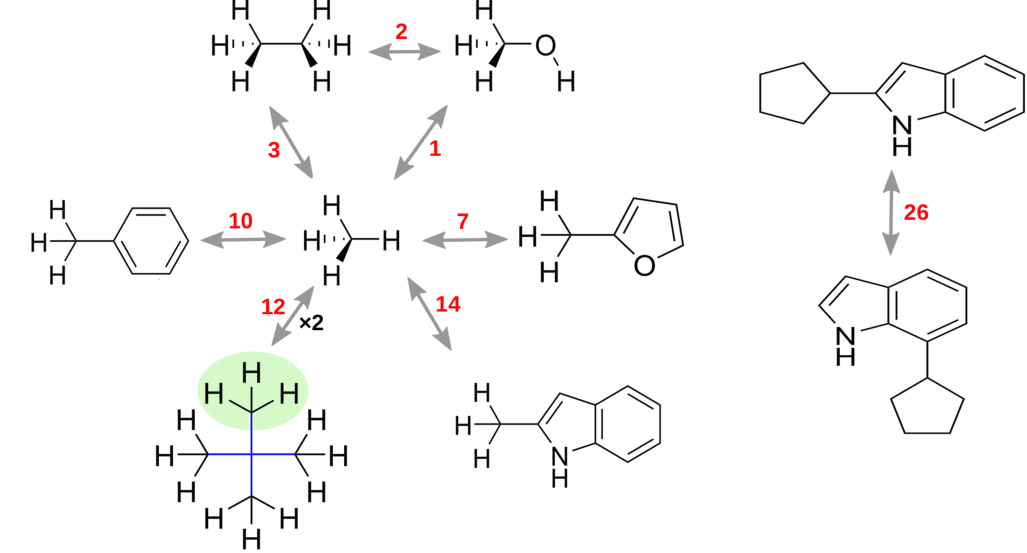
\includegraphics[width=\textwidth]{figures/cycles.pdf}
  \caption{The thermodynamic cycles considered in this study.  To
    compute the free energy of hydration, all pair--wise
    transformations have to be carried out once in solution and once
    in vacuum.  Green and blue colours in neopentane show two
    alternative mappings for methane.  The numbers in red denote the
    number of dummy atoms.}
  \label{fig:cycles}
\end{figure}
%DLM: I have the same problem as noted above with the methyls in this figure; it'd be really nice to make them look a little more chemical. To some extent also true for neopentane's central carbon I think.

The ethane $\rightarrow$ methanol transformation is traditionally
regarded as a standard test for RAFE
simulations~\cite{doi:10.1063/1.449208, doi:10.1021/jp981629f}.   The
other transformations are centered around mutations from and to
methane, and are meant to mimic components of typical transformations that could be attempted
in the context of e.g.\ protein--ligand binding calculations. The
2--cyclopentanylindole to 7--cyclopentanylindole (2--CPI to 7--CPI in our notation)
transformation has been added to include both deletion as well as
insertion of sub--parts of the perturbed group in one transformation, an aspect not tested by the other transformations.  For
neopentane $\rightarrow$ methane two
alternative mappings have been considered, see Fig.~\ref{fig:cycles}.  One mapping has methane matched to a terminal methyl (green) and the other
one has the methane carbon matched with the central carbon in
neopentane (blue).  The first approach will be called ``terminally mapped'' and
the second one ``centrally mapped''.


\subsection{Free Energy Simulation Protocols}
\label{sec:rafe_protocols}

One of the major goals of the present study is to ensure
consistency and reproducibility from the computational protocols.  This is complicated by the fact
that a given MD software may employ a range of methods and algorithms that one may not be
able to duplicate exactly with other MD software.
In particular, how the alchemical transformation is controlled via the coupling parameter may be very different.
At the most basic level, even pressure and temperature scaling, integrators and other algorithms can also display important differences.
It is unclear if and how any of these implementation details can affect results.
The implementation details of alchemical free energy simulation in code are discussed in subsection~\ref{sec:afe_impl}.

In this study we consider a set of simple organic molecules (see
Fig.~\ref{fig:cycles}).  As the focus here is on probing for
reproducibility among various MD packages, we chose fairly small,
rigid and neutral molecules to minimize statistical sampling errors, and
avoid difficulties with charged
particles~\cite{rocklin_calculating_2013, JCC:JCC1050}.  The force
field was chosen to be GAFF (version
1.8),~\cite{wang_development_2004} utilizing AM1/BCC charges~ for the solute,\cite{jakalian_fast_2000,jakalian_fast_2002} and
TIP3P for the solvent.~\cite{jorgensen_comparison_1983-1}
% REF: Durell, S. R.; Brooks, B. R.; Ben-Naim, A. J Phys Chem 1994, 98, 2198.
% REF Pettitt, B. M.; Karplus, M. Chem Phys Lett 1985, 121, 194.
%
% BR: ARE WE OR NOT ALL USING THE TIP3P with the small LJ on the hydrogens?
%
%CHARMM uses a slightly modified form of the TIP3P water model,50 which includes LJ param- eters for the hydrogens as well as the oxygen.48,51 The properties of the model are not significantly altered,52�54 because the hydrogens (rmin 5 0.2245 A? ) are well inside the van der Waals spheres of the oxygens (rmin 5 1.7682 A? , O H bond length 5 0.9572 A?). The modification was introduced to avoid singular- ities in the use of integral equations for representing the sol- vent55; it is not important for explicit-solvent MD simulations.
%
% REF: Durell, S. R.; Brooks, B. R.; Ben-Naim, A. J Phys Chem 1994, 98, 2198.
% REF Pettitt, B. M.; Karplus, M. Chem Phys Lett 1985, 121, 194.
%
Charges were computed with the \progname{antechamber} program and
missing bonded and vdW terms were generated with the
\progname{parmchk2} program, both from the AmberTools16 distribution.
All parameters are compiled at
https://github.com/halx/relative-solvation-inputs.
The quality of free energies of various small molecule force fields
has been discussed elsewhere, see
e.g.\ Refs.~\citenum{doi:10.1021/ct300203w, Hu2016}.

While the MD packages principally allow a ``one--step''
transformation~\cite{steinbrecher_soft-core_2011},
that is with both LJ and Coulombic parameters varied
simultaneously (unified protocol), it has also been proposed that carrying out a
split protocol may be more efficient.~\cite{Deng-2004, naden_linear_2014, naden_linear_2015}
In such a protocol the charges are transformed
linearly between the end states followed by a mutation of the van der
Waals parameters using a softcore
potential (see section~\ref{S-sec:softcores}x in the
SI for details) on the LJ term only.~\cite{beutler_avoiding_1994,
  zacharias_separationshifted_1994}  It is important to note that in the split protocol, charges have to be switched off before LJ parameters (and vice versa
for the transformation in opposite direction) to avoid collapse of
other atoms, e.g.\ solvents, onto a ``naked''
charge,\cite{pitera_comparison_2002, anwar_robust_2005,
steinbrecher_soft-core_2011} see section~\ref{S-sec:separated}x in the SI.

All simulations were started from simulation boxes prepared by
FESetup~\cite{loeffler_fesetup:_2015}.  During construction of the
perturbed systems, steric overlaps between the solute and the
solvent may happen.  This is because each unperturbed solute is independently
equilibrated but the final perturbed system combined from those, potentially
differently sized solutes.  To make the number of atoms the same for forward
and backward setups the water coordinates of the larger of the two boxes are
chosen.  Thus, in transformations from a smaller to a larger solute, water
molecules may be in close proximity to the solute.  At the end of the
construction process, FESetup performs a minimization onto the
system.  In addition, some simulation protocols started with a,
redundant, minimization step.  All production simulations were run at
\SI{298}{K} and \SI{1.0}{bar} in the NPT ensemble.  Water molecules
were constraint.  As specified below, some software performed a second
minimization of the system before proceeding with the alchemical free
energy calcualtion.  Atomic masses were not changed along the
alchemical transformations as this would affect only the kinetic
energy, and would not contribute to the free energy change.

%BR: I SUGGEST TO ORDER ALL THE ITEMS SIMILARLY FOR ALL THE PROGRAMS...
%\paragraph{PROGRAM.}
%
%Program and module used.
%Number of windows
%Starting coordinates of the windows
%Simulation length timestep
%SHAKE and CONSTRAINTS
%Temperature and pressure
%PME and cutoff of real-space ELEC part and vdW, swithing-shifting-truncation?
%Cutoff for the vacuum simulations
%Soft-core?
%Long Range Correction (LRC) term

\paragraph{AMBER.}
The AMBER16 program was used for this set of free energy calculations.
%
Typically 11 windows were used for charge mutations and 21 windows for VdW mutations.
In some instances, steep variations in gradients were observed with this protocol and additional windows were added to obtain smoother integration profiles.
The starting coordinates were usually taken directly from the pre--equilibrated setup step but no further $\lambda$ specific equilibration  was carried out,
i.e.\ RAFE MD simulations were started with new velocities appropriate for the final simulation temperature.
In a very few cases it was necessary to use coordinates from the end of the simulation at a nearby $\lambda$ state because of simulation instabilities.
This happened in transformations with a larger number of dummy atoms.
Absolute transformations were carried out using a one step protocol featuring 21 windows initially.
For some perturbations additional windows were run in regions where the free energy gradients varied sharply.
Each window was simulated for 2.5 ns, with the first 0.2 ns discarded prior analysis.
%
Water hydrogens (TIP3P) were constrained with SHAKE.
None of the atoms in the perturbed group where constrained and hence the time step was set to \SI{1}{fs}.
An alternative protocol with SHAKE on bonds that do not change during transformation and a time step of \SI{2}{fs} was also tested (see SOMD protocol below).
%
The temperature was controlled through a Langevin thermostat with a friction constant of \SI{2.0}{ps^{-1}} and pressure
rescaling through a Monte Carlo barostat with 100 steps between isotropic volume change attempts.
%
Long--range electrostatics in solution was handled with Particle Mesh Eward (PME) and an atom--based cutoff
of \SI{8.0}{\angstrom} for the real-space Coulomb and vdW interactions.
No cutoff was used for the vacuum simulations.
%
A Long Range Correction (LRC) term for truncated VdW interactions is applied during the MD simulations.
%

\paragraph{CHARMM.}
The version c40b1 was used for this set of free energy calculations.
The PERT module was used to handle the alchemical transformations.
%
Three different approaches were used to calculate the relative Gibbs free energy: (i) RAFE simulation where electrostatic and VdW interactions were changed separately (split-protocol) , (ii) RAFE simulation where electrostatic and VdW interactions were changed together (unified-protocol) , and (iii) difference between free energies from two AFE simulations where AFE simulations followed unified-protocol.
%
In total, 21 evenly spaced windows were used and all windows were run for \SI{1.5}{ns} with a timestep of \SI{1}{fs}.
Most windows used the same pre-equilibrated configuration.
A few windows at the end-points (involving hydrogen being transformed to heavy atom or vice versa) were unstable due to steric clashes with starting coordinates and were equilibrated using \SI{0.1}{fs} to \SI{0.5}{fs}.
%
Only water hydrogens (TIP3P) were constrained with SHAKE.
%
Conditions of constant temperature and pressure control were maintained using the Berendsen weak coupling method,
with a compressibility of \SI{4.63e-5}{atm^{-1}} and temperature and pressure coupling constants of \SI{5.0}{ps^{-1}}.
%
Long--range electrostatics in solution was handled with PME to order 6 with a cutoff of \SI{12.0}{\angstrom} for the real-space Coulomb and vdW interactions.
No cutoff was used for the vacuum simulations.
%
 No LRC term was applied during the alchemical MD simulations but a solute-solvent LRC term was included in post-processing to calculate the final free energy.
%
The PSSP softcore potential function was used for the perturbed atoms.
The PERT module currently does not currently support the force switching (option \inpopt{VFSwitch}) for LJ potentials with softcores.
The CHARMM PARAM27 force fields, however, is parameterized to use force switching \cite{JCC:JCC21287}.
Accordingly, we used the potential switching only (option \inpopt{VSwitch}) with an inner cutoff of \SI{10}{\angstrom} and outer cutoff of \SI{12}{\angstrom}.

\paragraph{GROMACS.}
GROMACS version 4.6.7 was used to carry out this set of free energy calculations.
%
Each transformation had its Gibbs free energy calculated:
(i) in a single topology approach in which LJ energy terms were changed separately from the electrostatic and bonded components;
(ii) in a single topology approach in which bonded, LJ, and electrostatic terms are changed together; and
(iii) via the difference between two absolute calculations.
In the first two cases, each alchemical transformation was described by 31 and 16 states, respectively, and simulated for \SI{4.2}{ns} with time steps of \SI{1.0}{fs} in water and vacuum.
We used a 20-step alchemical protocol where charge coupling and LJ coupling were dealt with separately along the path \cite{Mobley2014, doi:10.1021/acs.jced.7b00104}.
%
The free energies were calculated from \SI{5}{ns} Langevin dynamics at \SI{298}{K}.
A friction coefficient of \SI{1.0}{ps/m_{atom}} was used, where $m_{atom}$ is the the mass of the atom.
No holonomic bond or angle constraints were used.
A Parrinello--Rahman barostat with $\tau_p =$ \SI{10}{ps} and compressibility equal to \SI{4.5d-5}{bar^{-1}} was used.
%
Two methods were used to calculate electrostatic interactions:
Particle Mesh Ewald (PME) and charge group-based Reaction Field with a dielectric of 78.3, as implemented in the software.
PME calculations were of order 6 and had a tolerance of \num{1.0d-6}, with a grid spacing of \SI{1.0}{\angstrom}.
We set the real-space electrostatic and VdW cutoffs to \SI{10.0}{\angstrom}; a switch was applied to the latter starting at \SI{9.0}{\angstrom}.
A cutoff \SI{50.0}{\angstrom} was used for the vacuum simulations.
%
A Long Range Correction (LRC) term for truncated VdW interactions was applied during the MD simulations.
%
All transformations required the use of softcore potentials to avoid numerical problems in the free energy calculation.
We chose the 1--1--6 softcore potential for LJ terms ($\alpha$=0.5 and $\sigma$=0.3) for atoms whose parameters were being perturbed
and used the default softcore Coulomb implementation in paths where charges, LJ, and bonded terms were modified together,
but no soft core potentials were applied to Coulomb interactions when electrostatic interactions were modified separately.

\paragraph{SOMD.}
%Program and module used.
This set of free energy calculations was carried out with SOMD from the Sire 2016.1 release.~\cite{Sire-2016, doi:10.1021/ct300857j}
%Number of windows
Each alchemical transformation was divided into 17 evenly spaced windows and simulated for \SI{2}{ns} each both in water and in vacuum. The absolute hydration free energies were computed by annihilating non-bonded interactions of the solute in two steps. In the first step the free energy change for discharging the solute was computed. In the second step the free energy change for turning off the Lennard-Jones terms of the discharged solute was computed. Each step was carried out using 17 evenly spaced windows.
%Starting coordinates of the windows
The starting coordinates for each window were obtained by an additional energy minimization of the same pre-equilibrated and minimized configuration generated by FESetup.
%Simulation length timestep
A velocity-Verlet integrator was employed with a \SI{2}{fs} time step.
%SHAKE and CONSTRAINTS
Water hydrogens (TIP3P) were constrained with SHAKE. For the alchemical solute, only bonds involving hydrogens which are not alchemically transformed were constrained. This approach is referred as the ``unperturbed H bond constraint protocol''. Given the number of the perturbed hydrogen bonds in the solutes (Fig.~\ref{fig:cycles}, this constraint allows to use a \SI{2}{fs} time-step.
%Temperature and pressure
Temperature control was achieved with the Andersen thermostat,~\cite{doi:10.1063/1.439486} with a stochastic collision frequency of \SI{10}{ps^{-1}}.
A Monte Carlo barostat assured pressure control, with isotropic box edge scaling moves attempted every 25 time steps.
%PME and cutoff of real-space ELEC part and vdW, swithing-shifting-truncation?
A shifted atom--based Barker--Watts reaction field,~\cite{doi:10.1080/00268977300102101} with a dielectric constant of \num{78.3} was adopted for the solution phase simulations with a cutoff of \SI{10}{\angstrom}. A similar cutoff was used for LJ interactions.
%Cutoff for the vacuum simulations
The reaction field was not employed in the vacuum legs, where a Coulombic potential without cutoff was used.  A protocol to account for the different treatment of intramolecular electrostatics in vacuum and solution is described in the supporting information.
%Soft-core?
The softcore parameters (Eq.~S\ref{S-eq:general-softcore}x) were set to default values for all the transformations,
specifically $n = 0$ for Coulombic interactions and $\alpha = 2.0$ for the LJ potential~\cite{doi:10.1021/ct700081t}.
%Long Range Correction (LRC) term
Additionally, an end-point correction for truncated VdW potentials was applied by post-processing of end-state trajectories as described previously elsewhere.~\cite{shirtsLRC,BosisioHG}


\begin{table}[]
\centering
\caption{Summary of the technical details for the relative hydration free energy calculations carried out with the various codes.}
\label{tab:resumeSpecifications}
\makebox[\textwidth][c]{
\resizebox{0.7\width}{!}{
\begin{tabular}{lllll}
\hline
 &  AMBER & CHARMM & GROMACS & SOMD  \\                                                                                                                                             \hline
Version & AMBER16   & c40b1  & 4.6.7 & 2016.1 \\
Module  & \progname{pmemd, sander}  & \progname{PERT} & \progname{gmx} & \progname{somd-freenrg}\\
Protocol& Split protocol  & Unified protocol & Split protocol & Unified protocol\\
Number of $\lambda$ windows
	& \begin{tabular}[c]{@{}l@{}}11 (charge mutations)\\ 21 (vdW mutations)\end{tabular}                                                                            & 21 evenly spaced                                                                                                                                    & \begin{tabular}[c]{@{}l@{}}31 (charge mutations)\\ 31 (vdW mutations)\end{tabular}
	& 17 evenly spaced\\
Starting coordinates  & FESetup pre-equilibration   & FESetup pre-equilibration   & FESetup pre-equilibration   & FESetup pre-equilibration  \\
Simulation length per window & 2.5 ns  & 1.5 ns &  4.2 ns & 2 ns\\
Timestep& 1 fs  & 1 fs & 1fs & 2fs\\
Electrostatic method & PME   & PME & PME & atom-based RF\\
Solvated phase cutoff& 8 \AA{} & 12 \AA{} & 10 \AA{} & 10 \AA{}\\
Vacuum phase cutoff  & no cutoff & no cutoff & 50 \AA{} & no cutoff\\
Constraint  & none  & none & none & H-bonds not perturbed\\
LRC corrections   & during MD  & post-processing & during MD & post-processing\\
Barostat  & Monte Carlo & Berendsen & Parrinello-Rahman & Monte Carlo \\
Thermostat & Langevin   & Berendsen & Langevin          & Andersen \\
\\
Soft core parameters         & \begin{tabular}[c]{@{}l@{}}$r_{LJ}=(2\sigma_{ij}^6 \lambda + r_{ij}^6)^{1/6}$\\ \\ \\ $r_{Coul} = (\beta \lambda + r^p_{ij})^{1/p}$\\ \\ \\ $n=1$\end{tabular}
			     & \begin{tabular}[c]{@{}l@{}}$r_{LJ}=(2\lambda + r^2_{ij})^{1/2}$\\ \\ \\ $r_{Coul} = (\beta \lambda + r_{ij}^2)^{1/2}$\\ \\ \\ $n=1$\end{tabular}
			     & \begin{tabular}[c]{@{}l@{}}$r_{LJ} = (2\sigma_{ij}^{6}\lambda + r_{ij}^6)^{1/6}$\\ \\ \\ $r_{coul} = r_{LJ}$\\ \\ \\ $n=1$\end{tabular}
			     & \begin{tabular}[c]{@{}l@{}}$r_{LJ} = (2\sigma_{ij}\lambda +  r^2_{ij})^{1/2}$\\ \\ \\ $r_{Coul} = (\lambda + r^2_{ij} )^{1/2}$\\ \\ \\ $n=1$\end{tabular} \\
                             &                                                                                                                                                                &                                                                                                                                                     &                                                                                                                                         &                                                                                                                                                           \\ \hline
\end{tabular}%
}
}
\end{table}

\newpage

\subsection{Free Energy Estimations}
\label{sec:analysis}

In this work we primarily focus on TI as this is supported by all the
tested MD packages ``out--of--the--box''. Equation~\ref{eq:ti}
computes the free energy as \begin{equation}\label{eq:ti}
  \Delta G = \int_{\lambda=0}^{\lambda=1}
  \left\langle
  \frac{\mathscr{H}(\vec{q},\vec{p};\lambda)}{\partial\lambda}\right\rangle_\lambda
  d\lambda
\end{equation}
where $\mathscr{H}(\vec{q},\vec{p};\lambda)$ is the Hamiltonian as a
function of the coordinate vectors $\vec{q}$ and the momentum vectors
$\vec{p}$, and parametric dependence on the coupling parameter
$\lambda$ is explicit.  The angle brackets denote the ensemble average
of the gradient of the Hamiltonian with respect to $\lambda$, at a
given $\lambda$ value.  Results from additional
estimators will be given where available.  We have used the
\progname{alchemical analysis tool}~\cite{klimovich_guidelines_2015}
for all analyses.  This tool provides various estimators such as TI,
TI with cubic splines, BAR and MBAR.  We have used the cubic splines
method to integrate the free energy.  All data was sub--sampled to
eliminate correlated data~\cite{doi:10.1021/ct0502864}.

All RAFE simulations were run in triplicate in forward as well as
backward direction for a total of 6 simulations per mutation.  The
final hydration free energy $\Delta\Delta G_{\mathrm{hydr}}$ was
computed as the average for each direction separately.  For comparison we have also calculated the absolute (standard) hydration free energies for all molecules in Fig.~\ref{fig:cycles}.

To estimate the reliability and convergence of the results, the
standard error of the mean (SEM) has been calculated.  The SEM is
defined as
\begin{equation}
  \label{eq:sem}
  \mathrm{err}(\Delta\Delta G_{\mathrm{hydr}}) = \frac{\sigma}{\sqrt{n}}
\end{equation}
where $\sigma$ is the sample standard deviation of the three $\Delta \Delta G_{\mathrm{hydr}}$ values, and $n=3$.
%DLM: Add ref
For each free energy change the SEM was evaluated as:
\begin{equation}
  \label{eq:sem-comb}
  \mathrm{err}(\mathrm{combined}) = \sqrt{\sum_i \sigma_i^2}.
\end{equation}

We also make use of the mean absolute error MAE (also called mean unsigned
error, MUE) to compare data sets.
\begin{equation}
\label{eq:MUE}
\mathrm{MAE} = \frac{1}{N}\sum_\mathrm{i=1}^N \left | y_\mathrm{i} -
x_\mathrm{i} \right |
\end{equation}
where $N$ is the total number of samples, $y_\mathrm{i}$ and $x_\mathrm{i}$ are
the $i$--th datum to be compared.


\section{Results}
\label{sec:results}

In the following we will present our RAFE results for the
thermodynamic cycles shown in Fig.~\ref{fig:thermocycle}.  We will use
absolute hydration free energies here as our standard point of
comparison because for the present dataset they can be calculated with
high precision~\cite{doi:10.1021/acs.jced.7b00104}, and are simpler to
set up and implement than relative calculations.  Prior work has
successfully compared calculated absolute hydration free energies
across GROMACS and DESMOND codes.~\cite{klimovich_predicting_2010}

Tab.~\ref{tab:absolute2} summarizes results for the absolute hydration
free energies.  The table shows the data
from simulations with the recommended protocol for each MD code, as
discussed in detail in the following subsections.
The  precision of the calculated free energies is similar between
AMBER, CHARMM and GROMACS, whereas the SOMD free energies are less
precise.  This may reflect differences in the lambda schedules and
length of trajectories between the different codes.  Nonetheless the
standard errors are typically well under \SI{0.1}{kcal/mol}, thus it
becomes meaningful to investigate small differences of a few tenths of
\si{kcal/mol} between codes.

The $\Delta G_{\mathrm{hydr}}$
obtained with the various MD packages in
this way agree quite well given statistical errors, although some larger deviations are apparent as
well.  GROMACS predicts a smaller $\Delta G_{\mathrm{hydr}}$ for
methanol by about \SI{+0.2}{kcal.mol^{-1}}.  Similarly, there are some
small discrepancies in the toluene, 2--methylfuran and 2--methylindole
cases, where CHARMM produces slightly smaller $\Delta
G_{\mathrm{hydr}}$.  These small discrepancies may be due to the
differences in calculated densities between CHARMM and other codes
(typically smaller by ca.\ \SI{0.01}{g/cm^3}).
The largest deviation can be found for one of the largest
molecules (7--CPI) with the AMBER result being less negative than with
the other MD packages by 0.4--\SI{0.8}{kcal.mol^{-1}}.  This
particular discrepancy does not correlate with significant variations
in density between AMBER and other codes.

As an additional check we computed densities in the fully decoupled
states and compared the results to reported densities for a pure TIP3P
water box.  The average densities across all simulations are
\SI{0.980+-0.002}{g/cm^3}, \SI{0.973+-0.002}{g/cm^3},
\SI{0.979+-0.002}{g/cm^3}, \SI{0.976+-0.003}{g/cm^3} for AMBER,
CHARMM, GROMACS and SOMD respectively.  AMBER and GROMACS show higher
densities presumably because a LRC term was applied during the MD
simulations, whereas LRC terms for SOMD and CHARMM are only applied via
post-processing of trajectories.  For reference, a recent study from Lee--Ping et al.\ reports a
TIP3P water density of \SI{0.980}{g/cm^3}~\cite{doi:10.1021/jz500737m}.

\begin{table}[]
  \begin{minipage}{\linewidth}
    \caption{Absolute hydration free energies (in kcal/mol) and end-state densities  (in g/cm3) as obtained from AFE calculations. Uncertainties on the last decimal are given in parenthesis.}\label{tab:absolute2}
    \makebox[\textwidth][c]{
      \begin{tabular}{llrrrrrrr}
        \toprule
        \multicolumn{1}{c}{Solute}
        & \multicolumn{2}{c}{AMBER}
        & \multicolumn{2}{c}{CHARMM}
        & \multicolumn{2}{c}{GROMACS}
        & \multicolumn{2}{c}{SOMD} \\
        \multicolumn{1}{c}{ }
        & Free energy & Density
        & Free energy & Density
        & Free energy & Density
        & Free energy & Density   \\
        & (kcal/mol) & (g/cm$^3$)
        & (kcal/mol) & (g/cm$^3$)
        & (kcal/mol) & (g/cm$^3$)
        & (kcal/mol) & (g/cm$^3$)  \\
        \midrule
        methane  &
         2.47(1) & 0.986(1) &
         2.48(1) & 0.977(1) &
         2.44(1) & 0.987(1) &
         2.52(2) & 0.982(1) \\
        methanol  &
        -3.73(1) & 0.988(1) &
        -3.72(1) & 0.980(1) &
        -3.51(1) & 0.988(1) &
        -3.70(5) & 0.987(1) \\
        ethane  &
         2.50(1) & 0.988(1) &
         2.50(1) & 0.979(1) &
         2.48(1) & 0.988(1) &
         2.56(1) & 0.984(1) \\
        toluene  &
        -0.72(1) & 0.991(1) &
        -0.64(1) & 0.983(1) &
        -0.72(1) & 0.991(1) &
        -0.55(2) & 0.989(1) \\
        neopentane  &
         2.61(1) & 0.990(1) &
         2.58(2) & 0.981(1) &
         2.58(1) & 0.990(1) &
         2.71(6) & 0.987(1) \\
        2-methylfuran  &
        -0.49(2) & 0.991(1) &
        -0.42(1) & 0.983(1) &
        -0.51(1) & 0.991(1) &
        -0.39(2) & 0.989(1) \\
        2-methylindole  &
        -6.24(1) & 0.993(1) &
        -6.06(1) & 0.984(1) &
        -6.35(1) & 0.993(1) &
        -6.06(4) & 0.990(1) \\
        2-CPI  &
        -6.05(2) & 0.995(1) &
        -6.18(4) & 0.992(1) &
        -6.54(1) & 0.994(1) &
        -6.14(9) & 0.991(1) \\
        7-CPI  &
        -5.66(3) & 0.995(1) &
        -6.28(3) & 0.982(1) &
        -6.52(2) & 0.995(1) &
        -6.1(1) & 0.992(1) \\
     \bottomrule
      \end{tabular}
    }
  \end{minipage}
\end{table}

Tab.~\ref{tab:mue-absolute} shows the MAE between SOMD, GROMACS, AMBER and CHARMM. CHARMM produces figures that agree the most with other MD packages. The largest difference reaches \SI{0.2}{kcal.mol^{-1}} for SOMD and GROMACS. Variabilities between the codes may be partly explained by differences in densities due to different treatments of long range electrostatics and vdW interactions.

\begin{table}[]
 \begin{minipage}{\linewidth}
   \caption{Mean Absolute Error (MAE) (\SI{}{kcal.mol^{-1}}) between relative free energies obtained with the absolute protocol for the SOMD, GROMACS, AMBER and CHARMM packages.}\label{tab:mue-absolute}
   \makebox[\textwidth][c]{
     \begin{tabular}{lrrr}
       \toprule
       Package & GROMACS & AMBER & CHARMM\\
       \midrule
       SOMD    & \num{0.20+-0.03} & \num{0.13+-0.04} & \num{0.08+-0.02} \\
       GROMACS &                 & \num{0.19+-0.01} & \num{0.15+-0.01} \\
       AMBER   &                 &                & \num{0.12+-0.01} \\
       \bottomrule
     \end{tabular}
   }
 \end{minipage}
\end{table}

Having established the predictive value from absolute transformations we now turn to computing $\Delta\Delta G_{\mathrm{hydr}}$ from relative mutations.
Tab.~\ref{tab:relative} summarizes the results for the four MD packages.
Again the data is from the recommended protocol for each package (see detailed discussions in the following subsections).

\begin{table}[]
{\footnotesize
  \begin{minipage}{\linewidth}
    \caption{Comparison of relative free energies of hydration for various MD
      packages as obtained from absolute (AFE) and relative (RAFE) transformations via unified or split
      protocols.  The values deduced from AFE transformations (given in the first row) were taken from Tab. 1.
      Signs of the  backward transformation have been reverted to
      correspond to the forward transformation. }\label{tab:relative}
    \makebox[\textwidth][c]{
      \begin{tabular}{llrrrrr}
        \toprule
        \multicolumn{2}{c}{Transformation\footnote{\label{foot:transform}The values deduced from the AFE absolute of Table 1 are given first.}}
        & \multicolumn{2}{c}{AMBER\footnote{\label{foot:split}split protocol.}} & CHARMM\footnote{\label{foot:unified2}unified protocol.} & GROMACS\footref{foot:split} & SOMD\footref{foot:unified2} \\
        & & \multicolumn{1}{c}{implicit\footnote{\label{foot:impl}using either the implicit or the explicit dummy atom approach.}} & \multicolumn{1}{c}{explicit\footref{foot:impl}} & & & \\
        \midrule
        ethane & methane &                  & \num{-0.02+-0.01} & \num{-0.03+-0.01} & \num{-0.04  +- 0.01} & \num{-0.05+-0.02} \\
        ethane & methane & \num{0.02+-0.01} & \num{-0.13+-0.02} & \num{-0.09 +-         0.02} & \num{-0.04 +- 0.02} & \num{0.05+-0.02} \\
        methane & ethane & \num{0.00+-0.03} & \num{-0.19+-0.03} & \num{-0.04 +-         0.01} & \num{-0.02 +- 0.01} & \num{0.01+-0.06} \\ \hdashline

        methanol & methane &                  & \num{6.20+-0.01} & \num{6.20+-0.02} & \num{5.95 +- 0.01} & \num{6.21+-0.06} \\
        methanol & methane & \num{6.19+-0.01} & \num{6.20+-0.02} & \num{6.18 +-         0.01} &         \num{6.20 +- 0.01} & \num{5.99+-0.05} \\
        methane & methanol & \num{6.20+-0.03} & \num{6.15+-0.01} & \num{6.21 +-         0.01} & \num{6.20 +- 0.01} & \num{5.97+-0.04} \\     \hdashline

        ethane & methanol &                  & \num{-6.22+-0.01} & \num{-6.22+-0.02} & \num{-5.98  +- 0.01} & \num{-6.26+-0.05} \\
        ethane  & methanol & \num{-6.20+-0.01} & \num{-6.27+-0.01} & \num{-6.25         +- 0.01} & \num{-6.19 +- 0.01} & \num{-6.09+-0.03} \\
        methanol & ethane & \num{-6.20+-0.01} & \num{-6.25+-0.01} & \num{-6.28         +- 0.01} & \num{-6.19+- 0.01} & \num{-6.09+-0.02} \\ \hdashline

        toluene & methane &                  & \num{3.19+-0.01} & \num{3.12+-0.01} & \num{3.16 +- 0.01} & \num{3.07+-0.03} \\
        toluene & methane & \num{3.24+-0.02} & \num{3.39+-0.02} & \num{3.04 +-         0.02} & \num{3.21 +- 0.01} & \num{2.89+-0.09} \\
        methane & toluene & \num{3.42+-0.03} & \num{3.52+-0.03} & \num{3.09 +-         0.02} & \num{3.20 +- 0.01} & \num{3.06+-0.02} \\ \hdashline

        neopentane & methane &                  & \num{-0.13+-0.02} & \num{-0.11+-0.02} & \num{-0.14 +- 0.01} & \num{-0.19+-0.06} \\
        neopentane\footnote{\label{foot:cent}central mapping.} & methane &         \num{0.32 +-0.04} & \num{-0.03+-0.06} & \num{-0.35 +- 0.01} &         \num{-0.15 +- 0.02} & \num{-0.20+-0.05} \\
        methane\footref{foot:cent} & neopentane & \num{0.25+-0.03} &         \num{-0.07+-0.03} & \num{-0.24 +- 0.02} & \num{-0.16 +- 0.05} &         \num{-0.13+-0.05} \\
        neopentane\footnote{\label{foot:term}terminal mapping.} & methane &         \num{-0.13+-0.01} & \num{-0.12+-0.02} & \num{-0.56 +- 0.02} &         \num{-0.14 +- 0.01} & \num{-0.11+-0.01} \\
        methane\footref{foot:term} & neopentane & \num{-0.13+-0.03} &         \num{-0.12+-0.03} & \num{-0.40 +- 0.02} & \num{-0.18 +- 0.03} &         \num{-0.10+-0.06} \\ \hdashline

        2--methylfuran & methane &                  & \num{2.96+-0.02} & \num{2.90+-0.01} &  \num{2.95 +- 0.01} & \num{2.90+-0.03} \\
        2--methylfuran  & methane & \num{3.09+-0.01} & \num{3.10+-0.01} &         \num{2.84 +- 0.03} & \num{2.93 +- 0.05} & \num{2.92+-0.05} \\
        methane & 2-methyfuran  & \num{3.10+-0.03} & \num{3.15+-0.03} &         \num{2.84 +- 0.02} & \num{2.96 +- 0.01} & \num{2.83+-0.03} \\ \hdashline

        2--methylindole & methane &                  & \num{8.72+-0.01} & \num{8.53+-0.02} & \num{8.79 +- 0.02} & \num{8.57+-0.03} \\
        2--methylindole & methane & \num{8.78+-0.03} & \num{8.78+-0.04} &        \num{8.49 +- 0.01} & \num{8.73 +- 0.03} & \num{8.64+-0.06} \\
        methane & 2-methylindole & \num{9.14+-0.02} & \num{9.13+-0.03} &         \num{8.56 +- 0.02} & \num{8.74 +- 0.01} & \num{8.67+-0.08} \\ \hdashline

        2--CPI & 7--CPI &                  & \num{0.39+-0.04} & \num{-0.11+-0.04} & \num{0.02 +- 0.05} & \num{0.08+-0.14} \\
        2--CPI\footnote{\label{foot:partial}partial         re/discharge i.e.\ only the charges of the appearing and the         disappearing 5--rings are switched.} & 7--CPI &
        \num{0.36+-0.03} & \num{0.63+-0.06} & \num{-0.01 +- 0.01} & \num{-0.01         +- 0.03} & \num{-0.11+-0.07} \\
        7--CPI\footref{foot:partial} & 2--CPI &         \num{0.34+-0.05} & \num{0.50+-0.03} & \num{0.04 +- 0.01} & \num{-0.20         +- 0.04} & \num{-0.01+-0.08} \\

        \bottomrule
      \end{tabular}
    }
  \end{minipage}
}
\end{table}

We reviewed firstly internal consistency of the different codes with the computed absolute hydration free energies. For each implementation we counted the number of times a calculated relative free energy deviates from the difference in reference absolute hydration free energies by more than 0.1 kcal/mol. This is significantly above the estimated uncertainties in calculated free energies in most instances. According to this criterion, the AMBER explicit implementation is the least consistent (10 deviations), followed by AMBER implicit (6 deviations), SOMD (6 deviations), CHARMM (5 deviations), GROMACS (5 deviations). The perturbations that give a discrepancy are not the same across codes, for instance methane->toluene with AMBER explicit deviates from the reference absolute hydration free energies by 0.33 kcal/mol, but at most 0.04 kcal/mol with other codes. SOMD and GROMACS show deviations of ca. 0.25 kcal/mol for methanol->methane but this is not the case for AMBER (implicit or explicit) or CHARMM.

We next reviewed consistency between forwards and backwards relative hydration free energies. Again counting the number of deviations that exceed 0.1 kcal/mol indicates that AMBER explicit is the least consistent (3 deviations), followed by AMBER implicit (2 deviations), CHARMM (2 deviations), GROMACS (1 deviation), SOMD (1 deviation). The largest deviation is observed with AMBER implicit for 2-methylindole <-> methane (0.36 kcal/mol).

Next we compared relative free energies across packages.
CHARMM tends to show relative free energies with smaller values for a number of transformations:  neopentane, 2--methylfuran and 2--methylindole. SOMD displays smaller values $\Delta\Delta G_{\mathrm{hydr}}$ for the methanol and toluene transformations.  The largest discrepancy, however, is in the neopentane transformation with central mapping where AMBER with implicit dummy atoms is about \SI{0.5}{kcal.mol^{-1}} higher and CHARMM about \SI{0.2}{kcal.mol^{-1}} lower than the other two codes.  The
terminal mapped neopentane case reveals AMBER to be in line with GROMACS and SOMD while CHARMM's results deviate further.  AMBER deviates also quite strongly from the other codes in the cyclopentanyl indole cases.

The MAEs of the relative free energy simulations are presented in
Tab.~\ref{tab:mue-relative}.  They are on average slightly larger than the MAEs from the absolute simulations (Tab.~\ref{tab:mue-absolute}) and reach \SI{0.26}{kcal.mol^{-1}} for AMBER compared with CHARMM.

\begin{table}[]
 \begin{minipage}{\linewidth}
   \caption{MAE (in \si{kcal.mol^{-1}}) comparing relative free energies from
     relative simulations between SOMD, GROMACS, AMBER and
     CHARMM.}\label{tab:mue-relative}
   \makebox[\textwidth][c]{
     \begin{tabular}{lrrr}
       \toprule
       Package & GROMACS & AMBER & CHARMM \\
       \midrule
       SOMD    & \num{0.11+-0.01} & \num{0.23+-0.01} & \num{0.15+-0.01} \\
       GROMACS &                 & \num{0.16+-0.01} & \num{0.13+-0.01} \\
       AMBER   &                 &               & \num{0.26+-0.01} \\
       \bottomrule
     \end{tabular}
   }
 \end{minipage}
\end{table}

We also computed cycle closure errors from Tab.~\ref{tab:cycle-closure} for
the closed cycle ethane$ \rightarrow$ methanol $\rightarrow$ methane $\rightarrow$ ethane (see Fig.~\ref{fig:cycles}). The results are shown in Tab.~\ref{tab:cycle-closure}. Uncertainties were estimated by propagating uncertainties from the individual perturbations. AMBER explicit dummy and CHARMM are the only protocol consistent within uncertainty estimates, but the deviations observed with the other protocols are small. The largest discrepancy is observed with the GROMACS unified PME protocol, with the error just under \SI{0.2}{kcal/mol}.

\begin{table}[]
  \begin{minipage}{\linewidth}
    \caption{Cycle closure errors (in \si{kcal.mol^{-1}}) for  ethane$ \rightarrow$ methanol $\rightarrow$ methane
$\rightarrow$ ethane}\label{tab:cycle-closure}
    \makebox[\textwidth][c]{
      \begin{tabular}{lrrr}
        \toprule
        Package and Protocol & Closure Error \\
        \midrule
        AMBER implicit    & 0.07 $\pm$ 0.04  \\
        AMBER explicit    & 0.02 $\pm$ 0.05  \\
        GROMACS split reaction field  &  0.05 $\pm$ 0.02  \\
        GROMACS unified reaction field  &  0.13 $\pm$ 0.03  \\
        GROMACS split PME  &  0.04 $\pm$ 0.01  \\
        GROMACS unified PME  &  0.18 $\pm$ 0.03  \\
        CHARMM            &   0.01 $\pm$ 0.03   \\
        SOMD                &  -0.11 $\pm$ 0.08 \\
        \bottomrule
      \end{tabular}
    }
  \end{minipage}
\end{table}

Finally we also examined whether the codes reproduced consistent changes in mean box volumes between forward and backward transformations. We find that the codes are generally consistent with GROMACS giving the most precise volume changes, whereas SOMD gives the least precise volume changes (See Tab. S1 in the SI). This indicates that the barostats used by the different simulation packages relax volume fluctuations with different efficiency, or that they sample different volume fluctuations.

\subsection{AMBER}
\label{sec:amber-results}

Using AMBER for RAFE simulations has revealed several problems with the implementation.  Some bugs were identified and the developers have fixed those for AMBER16, e.g.\ energy minimization in \progname{sander} led to
diverged coordinates for mapped atoms.  For a single topology description,
however, it is necessary to have the same coordinates.  Other issues are that
vacuum simulations can only be carried out with the \progname{sander} program
because \progname{pmemd} cannot handle AFE simulations in vacuum as of this writing.  This will, however, be rectified in future
versions~\cite{doi:10.1021/acs.jctc.7b00102}.  A disadvantage of
\progname{sander} is that it cannot be used to simulate the $\lambda$ end
points,~\cite{doi:10.1021/ct400340s} such that the TI gradients need to be
extrapolated (minimum and maximum allowed $\lambda$s are 0.005 and 0.995).
Also, \progname{sander} considers the whole system as the perturbed
region while \progname{pmemd} restricts this to a user chosen atom selection.
This has obvious implications for performance~\cite{doi:10.1021/ct400340s}.

We also found that, in contrast to the other three codes, AMBER does not yield
correct relative free energies with the unified protocol, i.e.\
when all force field parameters are scaled simultaneously (see
Tab.~\ref{S-tab:amber-onestep}x). The issue becomes apparent when more than a few dummy atoms are involved, while the unified protocol works for the
smaller transformations (refer to Fig.~\ref{fig:cycles}).  The split RAFE
protocol and absolute free energies, however, are very close to the other MD
packages as demonstrated in Tab.~\ref{tab:amber-comp} below.

End point geometries appear to be another issue with AMBER simulations
in both solution and vacuum.  This is most obvious in the neopentane
$\rightarrow$ methane test case with central mapping (see
\nameref{sec:rafe_setup} and Fig.~\ref{fig:thermocycle}).
As shown in Fig.~\ref{S-fig:amber-dist}x, the methane end state exhibits
incorrect distances between the carbon and the four
attached hydrogens of approximately \SI{1.23}{\angstrom}.  This value is about
\SI{1.12}{\angstrom} for the terminal dummy atoms in the other test cases but
still higher than the expected \SI{1.09}{\angstrom} on average.
Fig.~\ref{S-fig:amber-dist}x demonstrates how this depends on the number of
dummy atoms immediately surrounding the central atom.

We also compare free energies obtained from the implicit dummy approach in
AMBER with results from explicit dummy atom simulations and results from
absolute transformations described in Tab.~\ref{tab:absolute2} and
\ref{tab:relative}.  The relative simulations have been carried out with the
split protocol while the absolute simulations used a unified protocol
throughout.  SHAKE was explicitly deactivated for all bonds in the perturbed
region in these protocols.  Tab.~\ref{tab:amber-comp} shows selected results
for transformations with SHAKE enabled for all bonds to hydrogens except those
bonds that change bond length during transformation.
\begin{table}[]
  \begin{minipage}{\linewidth}
  \caption{Comparing AMBER results for simulations with various split protocols.
    The emphasis is here on the data with SHAKE enabled and a time step of
    \SI{2}{fs} (last column).  Implicit, explicit and absolute protocols had
    SHAKE disabled and a time step of \SI{1}{fs}. Signs of the  backward
    transformation have been reverted to correspond to the forward
    transformation.}\label{tab:amber-comp}
  \makebox[\textwidth][c]{
  \begin{tabular}{llrrrr}
    \toprule
    &                & implicit & explicit & absolute & SHAKE\footnote{implicit
    dummy atom protocol with $\delta t =$ \SI{2}{fs} and SHAKE on all H--bonds
    except perturbed bonds.} \\
    \multicolumn{2}{l}{transformation}          & $\Delta\Delta G$  &
    $\Delta\Delta G$ & $\Delta G$ & $\Delta\Delta G$ \\
    \midrule
ethane  & methanol & \num{-6.20+-0.01} & \num{-6.27+-0.01} &
\multirow{2}{*}{\num{-6.22+-0.01}} & \num{-6.18+-0.01} \\
methanol & ethane & \num{-6.20+-0.01} & \num{-6.25+-0.01} & & \\
toluene & methane & \num{3.24+-0.02} & \num{3.39+-0.02} &
\multirow{2}{*}{\num{3.19+-0.01}} & \num{3.27+-0.03} \\
methane & toluene & \num{3.42+-0.03} & \num{3.52+-0.03} & & \\
neopentane\footnote{\label{foot:centA}central mapping.} & methane & \num{0.32
+-0.04} & \num{-0.03+-0.06} & \multirow{4}{*}{\num{-0.13+-0.02}} &
\num{0.35+-0.02} \\
methane\footref{foot:centA} & neopentane & \num{0.25+-0.03} & \num{-0.07+-0.03}
& & \\
neopentane\footnote{\label{foot:termA}terminal mapping.} & methane &
\num{-0.13+-0.01} & \num{-0.12+-0.02} & & \\
methane\footref{foot:termA} & neopentane & \num{-0.13+-0.03} &
\num{-0.12+-0.03} & & \\
    \bottomrule
  \end{tabular}
}
  \end{minipage}
\end{table}

The time step has been increased from \SI{1}{fs} as used in the other
three protocols to \SI{2}{fs}.  As the results are essentially the same as the
non--SHAKE simulations, this SHAKE protocol appears to be a viable solution to
increase the performance of RAFE simulations.  We have repeated this protocol
with AMBER in response to the results obtained with SOMD using this
implementation.  From a practical point of view, AMBER uses an \emph{atom}
based mask for bond SHAKEs such that the mask must be set for the hydrogens in
question while the same is not possible for their non--H counter--part in the
other state because \emph{all} bonds emanating from this atom would be affected.

In general, the free energies computed with each approach are in good agreement
with each other and with the results of the other MD packages
(Tab.~\ref{tab:absolute2} and \ref{tab:relative}).  There are, however, a few
notable deviations.  Neopentane $\rightarrow$ methane with central mapping
differs from the result with terminal mapping by about
\SI{0.4}{kcal.mol^{-1}}.  The terminal mapping and the free energies from the
explicit dummy simulations are, however, consistent with the absolute
transformations (Tab.~\ref{tab:absolute2}).  We also observe a systematic
deviation between forward and backward vacuum transformations in the
2--methylindole simulation (see Tab.~\ref{S-tab:amber-disc}x).  The gradient
is consistently shifted by 0.2--\SI{0.4}{kcal.mol^{-1}} for each $\lambda$ step
of the vdW plus bonded transformation with both implicit and explicit dummy
atoms.


\subsection{CHARMM}
\label{sec:charmm-results}

CHARMM for alchemical free energy calculation (AFE) has been widely used with PERT module, but few bugs not previously reported in CHARMM c40b1 were found and careful AFE setup is needed to produce robust and accurate results. Bugs regarding TI gradient accumulation in the parallel version were identified and fixed by Dr. Stefan Boresch.
The PERT module does not allow a hydrogen bond constraint (SHAKE) to be applied on the perturbed region, and this requires end point lambdas to be equilibrated carefully. These windows at end-point lambda were started with their own equilibration using timesteps of \SI{0.1}{fs} to \SI{0.5}{fs} before the production run. The VSwitch option was used to apply a switching function to the potential since that option is cannot be applied to forces for calculations run with the PERT module.

%, since the PERT module is not compatible with the VFSwitch %option that is a switching function applied to force.
%JM do we need to mention the above sentence?

The PSSP softcore potential function cannot handle Long-Range Correction (LRC) correctly. This effect is not clearly shown when the initial and final states are comparable in size, but the deviation becomes larger for perturbations that involve large changes in solute size, or for absolute alchemical free energy calculations. It is necessary to disable the LRC to obtain consistent free energies from relative and absolute alchemical free energy calculation protocols (see SI for details).

Tab. \ref{tab:charmm-results} shows the relative free energies obtained from CHARMM simulations.
\begin{table}[]
  \begin{minipage}{\linewidth}
  \caption{Comparing CHARMM results for simulations with various split protocols. Signs of the  backward
    transformation have been reverted to correspond to the forward
    transformation.}\label{tab:charmm-results}
  \makebox[\textwidth][c]{
  \begin{tabular}{llrrr}
    \toprule
     \multicolumn{2}{c}{\multirow{2}{*}{transformation}}  & \multicolumn{1}{c}{split} & \multicolumn{1}{c}{unified} & \multicolumn{1}{c}{absolute(unified)}  \\
     & &  \multicolumn{1}{c}{$\Delta\Delta G$}  & \multicolumn{1}{c}{$\Delta\Delta G$} & \multicolumn{1}{c}{$\Delta\Delta G$} \\
    \midrule
ethane  & methane & \num{-0.09+-0.01} & \num{-0.09+-0.02} & \multirow{2}{*}{\num{-0.03+-0.01}}  \\
methane & ethane & \num{-0.04+-0.01} & \num{-0.04+-0.01} &  \\
methanol & methane & \num{6.20+-0.01} & \num{6.18+-0.01} & \multirow{2}{*}{\num{6.20+-0.01}}  \\
methane & methanol & \num{6.30+-0.01} & \num{6.21+-0.01} &  \\
ethane  & methanol & \num{-6.21+-0.01} & \num{-6.25+-0.01} & \multirow{2}{*}{\num{-6.22+-0.02}}  \\
methanol & ethane & \num{-6.25+-0.01} & \num{-6.28+-0.01} &  \\
toluene & methane & \num{3.22+-0.01} & \num{3.04+-0.02} & \multirow{2}{*}{\num{3.12+-0.01}}  \\
methane & toluene & \num{3.28+-0.01} & \num{3.09+-0.02} &  \\
neopentane\footnote{\label{foot:centAX}central mapping.} & methane & \num{-0.29 +-0.01} & \num{-0.35+-0.01} & \multirow{4}{*}{\num{-0.11+-0.02}}  \\
methane\footref{foot:centAX} & neopentane & \num{-0.15+-0.01} & \num{-0.24+-0.02} &  \\
neopentane\footnote{\label{foot:termAX}terminal mapping.} & methane & \num{-0.42+-0.01} & \num{-0.56+-0.02} &  \\
methane\footref{foot:termAX} & neopentane & \num{-0.31+-0.01} & \num{-0.40+-0.02} &  \\
2-methylfuran & methane & \num{2.87+-0.01} & \num{2.84+-0.03} & \multirow{2}{*}{\num{2.90+-0.01}}  \\
methane & 2-methylfuran & \num{2.93+-0.01} & \num{2.84+-0.02} &  \\
2-methylindole & methane & \num{8.88+-0.01} & \num{8.49+-0.01} & \multirow{2}{*}{\num{8.53+-0.02}}  \\
methane & 2-methylindole & \num{8.81+-0.01} & \num{8.56+-0.02} &  \\
2-CPI & 7-CPI & \num{-0.02+-0.01} & \num{-0.01+-0.01} & \multirow{2}{*}{\num{-0.11+-0.04}}  \\
7-CPI & 2-CPI & \num{-0.01+-0.01} & \num{0.04+-0.01} &  \\
    \bottomrule
  \end{tabular}
}
  \end{minipage}
\end{table}
While results from all three protocols (split, unified, absolute) seem to be in good agreement with each other, the split-protocol results are more precise due to the additional amount of data generated. It is notable that the split-protocol results are more similar to the ones obtained by other MD packages (i.e. neopentane and toluene), but the relative-unified results are more consistent with the CHARMM absolute simulations (e.g. 2-methylindole). Overall, the relative free energies obtained by these three different protocols are in good agreement with those reported for the other MD packages (Tab. 1 and 3).

\subsection{GROMACS}
\label{sec:gromacs-results}

GROMACS has some run input options which can simplify the procedure
for setting up free energy calculations.  Specifically, \inpopt{couple-moltype}
implicitly defines the initial and final states by giving a special tag to a
molecule and controls whether intramolecular interactions of the tagged
molecule are retained or not along the alchemical path.  It should be used in
absolute free energy calculations to tag the molecule which will be decoupled
from the rest of the system.
Using this in relative calculations is possible, but will result in unintended
behavior and errors. The keywords \inpopt{couple-lambda0} and
\inpopt{couple-lambda1} control the interactions of the molecule specified by
\inpopt{couple-moltype} with its surroundings.
The entries \inpopt{vdw-lambdas} and \inpopt{fep-lambdas}
define the lambda schedule.  The former indicates the value of the $\lambda$
vector component that modifies van der Waals interactions for each state,
while the latter changes all $\lambda$ vector components that are not specified
in the \inpopt{.mdp} file.  For instance, in split protocol simulations, these
entries are sets such that the components of the energy are modified in
different stages.  If the transformation involves particle deletion (``forward
process''), \inpopt{fep-lambdas} is set to change charges and bonds
before \inpopt{vdw-lambdas} changes van de Waals components.
If the process involves particle insertion (``backward process'') we reverse
the roles.  In this work, \inpopt{mass-lambdas} were all set to zero  to avoid
mass changes during the the free energy calculations.  Unified protocols set all $\lambda$ vectors the same.

Tab. \ref{tab:groresults} lists the relative free energies obtained from
GROMACS simulations.
\begin{sidewaystable}[]
  \centering
  \caption{Relative hydration free energies obtained from GROMACS simulations
  in $kcal\cdot mol^{-1}$. Signs of the backward transformation have been
  reverted to correspond to the forward transformation.}
  \label{tab:groresults}
  \resizebox{\columnwidth}{!}{%
    \begin{tabular}{@{}rrrrrrrr@{}}
    \toprule
    &  & \multicolumn{2}{c}{split\footnote{results obtained
    from alchemical transformations with electrostatic and bonded scaling
    separate from vdW  parameter change.}} &
    \multicolumn{2}{c}{unified\footnote{results obtained from
    alchemical transformation
    with all parameters scaling together.}} &
    \multicolumn{2}{c}{absolute\footnote{results obtained from
    absolute free energy
    calculations.}} \\
    \multicolumn{1}{c}{} & \multicolumn{1}{c}{} & \multicolumn{1}{c}{RF} &
    \multicolumn{1}{c}{PME} & \multicolumn{1}{c}{RF} & \multicolumn{1}{c}{PME}
    & \multicolumn{1}{c}{RF} & \multicolumn{1}{c}{PME} \\
    \multicolumn{2}{c}{transformation} & \multicolumn{1}{c}{$\Delta \Delta G$}
    & \multicolumn{1}{c}{$\Delta \Delta G$} & \multicolumn{1}{c}{$\Delta \Delta
    G$} & \multicolumn{1}{c}{$\Delta \Delta G$} & \multicolumn{1}{c}{$\Delta
    \Delta G$} & \multicolumn{1}{c}{$\Delta \Delta G$} \\ \midrule
    ethane & methane & \num{-0.025 +- 0.005} & \num{-0.035 +- 0.02} &
    \num{-0.017 +- 0.003} & \num{-0.030 +- 0.001} & \num{-0.06 +- 0.01} &
    \num{-0.04 +- 0.01} \\
    methane & ethane & \num{-0.01 +- 0.02} & \num{-0.02 +- 0.01} & \num{0.046
    +- 0.02}\footnote{\label{foot:inv} inverted sign} & \num{0.01 +- 0.02} &
    &  \\
    methanol & methane & \num{6.163 +- 0.006} & \num{6.197 +- 0.004} &
    \num{7.30 +- 0.02} & \num{7.380 +- 0.007} & \num{5.77 +- 0.01} & \num{5.95
    +- 0.01} \\
    methane & methanol & \num{6.168 +- 0.005} & \num{6.199 +- 0.008} &
    \num{7.09 +- 0.02} & \num{7.17 +- 0.02} &  &  \\
    ethane & methanol & \num{-6.123 +- 0.007} & \num{-6.185 +- 0.006} &
    \num{-7.117 +- 0.005} & \num{-7.21 +- 0.02} & \num{-5.83 +- 0.01} &
    \num{-5.98 +- 0.01} \\
    methanol & ethane & \num{-6.124 +- 0.005} & \num{-6.193+- 0.004} &
    \num{-7.338 +- 0.004} & \num{-7.404 +- 0.004} &  &  \\
    toluene & methane & \num{3.22 +- 0.01} & \num{3.211 +- 0.006} & \num{3.229
    +- 0.008} & \num{3.22 +- 0.01} & \num{2.97 +- 0.01} & \num{3.16 +- 0.01} \\
    methane & toluene & \num{3.25 +- 0.01} & \num{3.20 +- 0.01} & \num{3.22 +-
    0.01} & \num{3.211 +- 0.001} &  &  \\
    neopentane\footnote{\label{foot:c-map}central mapping} & methane &
    \num{-0.103 +- 0.008} & \num{-0.15 +- 0.02} & \num{-0.08 +- 0.02} &
    \num{-0.18 +- 0.03} & \num{-0.18 +- 0.01} & \num{-0.14 +- 0.01} \\
    methane\footref{foot:c-map} & neopentane & \num{-0.11 +- 0.02} & \num{-0.16
    +- 0.05} & \num{0.00 +- 0.03} & \num{-0.18 +- 0.03} &  &  \\
    neopentane\footnote{\label{foot:t-map}terminal mapping} & methane &
    \num{-0.116 +- 0.007} & \num{-0.13 +- 0.01} & \num{-0.14 +- 0.01} &
    \num{-0.14 +- 0.01} &  &  \\
    methane\footref{foot:t-map} & neopentane & \num{-0.10 +- 0.03} &
    \num{-0.18 +- 0.03} & \num{-0.089 +- 0.007} & \num{-0.15 +- 0.02} &  &  \\
    2-methylfuran & methane & \num{2.986 +- 0.006} & \num{2.930 +- 0.05} &
    \num{3.05 +- 0.01} & \num{3.00 +- 0.01} & \num{2.87 +- 0.01} & \num{2.95 +-
    0.01} \\
    methane & 2-methylfuran & \num{3.007 +- 0.004} & \num{2.96 +- 0.01} &
    \num{3.056 +- 0.006} & \num{3.01 +- 0.01} &  &  \\
    2-methylindole & methane & \num{8.71 +- 0.02} & \num{8.73 +- 0.03} &
    \num{8.73 +- 0.01} & \num{8.80 +- 0.03} & \num{8.44 +- 0.02} & \num{8.79 +-
    0.02} \\
    methane & 2-methylindole & \num{8.73 +- 0.03} & \num{8.74 +- 0.01} &
    \num{8.30 +- 0.02} & \num{8.77 +- 0.04} &  &  \\
    2-CPI & 7-CPI & \num{-0.07 +- 0.02} &
    \num{-0.03 +- 0.03} & \num{-0.10 +- 0.05} & \num{-0.2 +- 0.1} & \num{-0.02
    +- 0.05} & \num{0.02 +- 0.02} \\
    7-CPI & 2-CPI & \num{-0.12 +- 0.06} &
    \num{-0.20 +- 0.04} & \num{-0.04 +- 0.06} & \num{-0.14 +- 0.09} &  &  \\
    \bottomrule
    \end{tabular}
  }
\end{sidewaystable}
Relative free energies are in good agreement with each other and with
$\Delta \Delta G_{\mathrm{hydr}}$ obtained from the other software used in this
study (Tab.~\ref{tab:absolute2} and \ref{tab:relative}).  A noteworthy
exception is the difference between the unified and split results of methane
$\rightarrow$ methanol and its reverse process. This was investigated further with
additional split protocol simulations using Coulomb softcore potentials (Tab.
\ref{tab:eff-sc}).
%DLM: This wording may need adjusting because it sounds like we've resolved the issue by this additional investigation, but in fact the additional investigation does nothing to resolve it, unless I'm missing something.
%GDRM: Can you explain? I wrote the paragraph under this table to address it. Or have I misunderstood the question?

\begin{table}[]
\centering
\caption{Relative hydration free energies of methanol $\rightarrow$ methane and
methane $\rightarrow$ methanol transformations without and with the use of
Coulomb softcore potentials from GROMACS. Signs of the backward
transformation have been reverted to correspond to the forward transformation.
The complete version of this table is in the SI.}
\label{tab:eff-sc}
\begin{tabular}{@{}llclclcl@{}}
\toprule
 &  & \multicolumn{2}{c}{split} & \multicolumn{2}{c}{split+sc} &
 \multicolumn{2}{c}{absolute} \\
 &  & RF & \multicolumn{1}{c}{PME} & RF & \multicolumn{1}{c}{PME} & RF &
 \multicolumn{1}{c}{PME} \\
\multicolumn{2}{c}{transformation} & $\Delta \Delta G$ &
\multicolumn{1}{c}{$\Delta \Delta G$} & $\Delta \Delta G$ &
\multicolumn{1}{c}{$\Delta \Delta G$} & $\Delta \Delta G$ &
\multicolumn{1}{c}{$\Delta \Delta G$} \\ \midrule
methanol & methane & \multicolumn{1}{l}{\num{6.163 +- 0.006}} & \num{6.197 +-
0.004} & \multicolumn{1}{l}{\num{7.32+-0.03}} & \num{7.42+-0.04} &
\multicolumn{1}{l}{\num{5.77 +- 0.01}} & \num{5.95 +- 0.01} \\
methane & methanol & \multicolumn{1}{l}{\num{6.168 +- 0.005}} & \num{6.199 +-
0.008} & \multicolumn{1}{l}{\num{7.14+-0.03}} & \num{7.21+-0.03} &
\multicolumn{1}{l}{} &  \\ \bottomrule
\end{tabular}
\end{table}

We noticed a difference of approximately \SI{1.5}{kcal.mol^{-1}} between the
split protocol without Coulomb softcore potentials and both protocols that
use it.  The data shown in Fig. \ref{S-fig:gro_sc_eff}x suggests that
softening of the electrostatic interactions requires adjustments in
the $\lambda$-distance between states in the rapidly varying part of
the $\partial \mathcal{H}/\partial\lambda$.  A variant that combined
the bonded terms with the vdW transformation did not change this
result.  Thus, we find that the split protocol without Coulomb
softcore potentials is the most effective way to calculate relative
free energies with the current GROMACS implementation.

Additionally it is worth mentioning is that relative free energy
simulations that feature alchemical transformations of a hydrogen atom
into a heavy atom will crash if the bond involving the hydrogen atom
is constrained with algorithms such as SHAKE or LINCS.  Successful
simulations require turning off the bond constraint and decreasing the
time step to 1 fs. Alternative protocols that require some scripting
and changes in the topology file could be pursued in the future. For
instance 2 fs constraints protocols similar to those used in SOMD or
AMBER in this study could be implemented via the definition of a new
atom type for alchemically perturbed hydrogen atoms.


\subsection{SOMD}
\label{sec:somd-results}

Fig.~\ref{S-fig:sire_histogram}x compares relative free energy of hydration
$\Delta\Delta G$ according to the protocol with unperturbed H bond constraints, with relative
$\Delta \Delta G$ obtained from two absolute free energy calculations.
Tab.~\ref{tab:relative} summarizes all the computed relative free energy of
hydration for the dataset in Fig.~\ref{fig:cycles}.
A very good agreement is observed between both methodologies
($R^2$=\SI{0.99+-0.01}{} and MAE = \SI{0.10+-0.03}{kcal.mol^{-1}}),
highlighting internal consistency within SOMD.

To achieve this level of reproducibility within SOMD it was crucial to pay close attention to constraints. Specifically, bonds that involve unperturbed hydrogen atoms are constrained. Bonds involving hydrogen atoms that are perturbed to a heavy element are unconstrained.  Additionally the atomic mass of the perturbed hydrogen atom is set to the mass of the heavy atom it is
perturbed to.  Bonds involving hydrogen atoms that are perturbed to another hydrogen atom type are constrained. We stress that it is acceptable to artificially increase the atomic mass of hydrogen atoms because the calculated excess free energy changes do not depend on atomic masses.

This protocol suppresses high frequency vibrations in flexible bonds involving hydrogen atoms, thus enabling a time
step of \SI{2}{fs}, whilst giving essentially negligible errors due to the use of constraints for perturbed bonds.  This is apparent from the comparison with the absolute hydration free energy calculations.  Additionally, the protocol
yields relative hydration free energy very similar  (MAE =
\SI{0.09}{kcal.mol^{-1}}) to those computed from simulations where noconstraints are applied on the solutes and a timestep of \SI{1}{fs} is used (See Fig.~\ref{S-fig:sire_constraints}x).

By contrast, a protocol that constrains all bonds in a solute leads to
significant differences with the absolute hydration free energies. For instance
neopentane $\rightarrow$ methane (centrally mapped) gives a RAFE
$\Delta\Delta G$=\SI{2.04 +- 0.01}{kcal.mol^{-1}}  whereas the absolute
hydration free energy calculations give $\Delta\Delta
G$=\SI{-0.19+-0.06}{kcal.mol^{-1}} as shown in
Tab.~\ref{S-tab:sire_constraints}x and fig.~\ref{S-fig:sire_constraints}x.

This discrepancy occurs because in the SOMD implementation, the energies of constrained bonds are not evaluated, but the calculation of the energies of the solute at perturbed $\lambda$ values is carried out using the coordinates of the reference $\lambda$ trajectory. This leads to a neglect of contributions of
the bonded term (and associated coupled terms) to the free energy change. The effect is more pronounced for perturbations that feature a large change in equilibrium bond lengths, such as those where a hydrogen atom is perturbed
to/from a heavy atom.

The reaction fields implemented in SOMD and GROMACS differ somewhat (atom-based
shifted Barker Watts,~\cite{doi:10.1080/00268977300102101} vs group based switched Barker Watts), but nevertheless SOMD and GROMACS RF produce comparable results with a MAE of \SI{0.18}{kcal.mol^{-1}}. Overall, the SOMD free energy estimations are in good agreement with the other MD packages, as the MAE suggests (see Tab.~\ref{tab:mue-relative}). For the methane $\rightarrow$ neopentane transformations SOMD yields consistent results between central and terminal mappings, as shown in Tab.~\ref{S-tab:sire-finalresults}x.
Reaction field and PME results are in good agreement.  All SOMD RAFE simulations were carried out with simultaneous transformation of Lennard-Jones, charges, and bonded terms. This suggests that the failure of the GROMACS ``unified protocol'' in some instances may be due to differences in the softcore Coulomb implementations.


\section{Discussion and Conclusions}
\label{sec:discuss}

This study addressed whether contemporary MD packages such as AMBER, CHARMM, GROMACS and SOMD are able to reproduce relative alchemical free energies of hydration for a set of neutral small organic molecules, given a
pre--defined force field.
We have found that establishing a simulation protocol that leads to consistent results across codes has been cumbersome due to technical difficulties encountered with every code.
This was the case despite our best efforts to maintain fairly consistent protocols for settings which were expected to significantly impact results.
For example, we used nominally the same form of soft core potentials in most of the codes compared , and implementations of many other algorithms which should be the same or are thought to be equivalent.
Still, we encountered numerous difficulties.
Overall, the MD codes have a wide range of options and setup features which makes it difficult for the unexperienced user to decide on the most
appropriate ones.

The free energies we have computed appear to be in reasonably good agreement with each other (see Tab.~\ref{tab:absolute2} and \ref{tab:relative}).  The average MAE between all codes \SI{0.14}{kcal/mol} for absolute free energies and \SI{0.17}{kcal/mol} for relative free energies.  This can be interpreted as the current ``limit of reproducibility'' for the field.  We have found viable protocols for each MD code to achieve
this level of reproducibility.  There is some doubt, however, over the AMBER
results because the particular version of the software we tested  cannot reproduce the correct end-point
geometries.  This is particularly evident in the neopentane to methane case
with central mapping where also the relative free energies are clearly
different from the other packages.  We suspect these issues reflect a bug in
the AMBER package but have been unable to isolate it; we have reported the
issue to the AMBER developers.

We were unable to define  a \emph{universal} protocol that could be recommended for use with all four codes.  Unified protocols do not appear to work with AMBER and GROMACS while SOMD and CHARMM had no problem in this regard.  We cannot rule out that the problem may lie e.g.\ only with the
vacuum leg of the thermodynamic cycle.  In the case of AMBER the vacuum simulation has currently been done with the separately developed \progname{sander} module.  The problem may be a consequence of the different softcore functions (see Eq.~S\ref{S-eq:general-softcore}x) used in these MD packages but further investigations are needed to resolve this issue.

The unperturbed H bond protocol is an interesting alternative which
applies constraints to all non--transforming bonds and thus allowed us
to increase the time step to \SI{2}{fs}.  The split protocol was found
to work well for all codes.  It appears to be the most effective
approach for GROMACS as shown with the methanol to methane case
because the unified protocol produces a less smooth
function~\cite{shirts_chapter_2007}.  A complete separation of lambdas
may not be necessary though as a certain degree of overlap between vdW
and Coulumb $\lambda$ may be a viable
solution~\cite{procacci_fast_2014} for equilibrium AFEs.

Comparison between codes is hampered by several factors.  Firstly, the codes use different simulation algorithms e.g.\
electrostatics are handled differently in vacuum i.e.\ infinite cutoff vs.\
reaction field.  Temperature and pressure control, time step integrators, etc. are other examples.  But the data here suggest that, if there are any systematic errors introduced through these algorithms, then they are small.  It is reassuring that AFEs for the systems tested here show only a small dependence on MD protocol decisions (provided a correct implementation).

Some of the differences between protocols used in this comparison could have been avoided, and it may be worth pursuing these in follow up work.
For example, the number of lambda values, length of simulations, and choice of Lennard-Jones cutoff were varied across packages in some cases.
While previous studies have suggested results are relatively insensitive to these choices, it may be worth further exploring these issues in follow-up work to ensure results are robust with respect to these settings.

To aid with follow-up studies, we make our input data and protocols available.  We recommend using this dataset to test and benchmark future RAFE implementations to validate reproducibility against other simulation packages.
Where possible, we recommend comparing results from both absolute and relative transformations to verify internal consistency.
The relative transformation should be run in both forward and backward directions, even if the free energy estimator is agnostic to this decision, as other implementation details (e.g. bugs in parameters, atomic masses) may lead to inconsistent results.

More specifically, various issues with current code bases have been revealed through this work.
We have found that constraints in connection with varying bond length can cause errors with GROMACS, just as masses must not be allowed to vary in RAFE simulations, both to avoid crashes and incorrect results from the
software.  CHARMM has issues with constraints and the PSSP softcores, and the PERT module cannot make use of the force switch as it is now standard for CHARMM force fields. Care must be taken when using the LRC long range correction keyword to avoid producing inconsistent results.  AMBER's problem with end point geometries and unified protocols has been pointed out above.

Another question is the ease of use of the different software.  For example, when a mutation entails both appearing and disappearing parts in split
protocols there is the problem of intermediates having a non--integral total
charge on the molecule.  An alternative would be to totally discharge and then
recharge the whole molecule which
would have the advantage of eliminating one additional evaluation of the reciprocal sum in PME~\cite{doi:10.1021/ct400340s}.
%JM is this going to make a significant difference in compute cost??? I don't think so so I don't see any advantage.
 However this is not attractive as this could significantly increase the sampling needed to obtain converged free energy changes.

 Another practical issue is the complex setup associated with the
 split protocol. For instance in GROMACS it is necessary to carry out two separate simulations per lambda because discharging and recharging groups cannot be selected separately.
Lambda paths as implemented in GROMACS could also be beneficial for other codes as they make the setup of split protocols easier.  The alternative we have used in codes lacking this feature is to mimic this protocol through careful construction of
topologies via scripting.

It may seem remarkable that of the computed free energies, the absolute hydration free energies seem to be more reproducible across codes than relative free energies.
Conventional wisdom is that relative free energy calculations are computationally less demanding than absolute free energy calculations, which would lead to the opposite result.
However, absolute calculations are considerably simpler to implement and deploy correctly as they do not involve as many challenging technical issues such as atom mapping, and the lambda protocols which must be employed have been optimized fairly well, since such calculations always involve either removal or insertion of atoms but never both simultaneously.
This has made absolute calculations valuable as large-scale tests of free energy methods and force fields (e.g.~\cite{Mobley2014, doi:10.1021/ct300203w} and others), and in the SAMPL series of blind challenges (e.g.~\cite{fennell_fixed-charge_2014, geballe_sampl3_2012}).
Thus absolute calculations are already well automated, robust across codes, and well-performing protocols are available.
Apparently similar is yet needed for relative free energy calculations.

The primary focus of this work was to achieve low statistical errors
to establish if codes are able to reproduce free energies.  We have
not investigated in detail the efficiency of the respective protocols
as this would require further, complex investigations.  For absolute
calculations the most demanding protocol and most precise protocol is
GROMACS (200 million aggregate time--steps per solute, average SEM
\SI{0.011}{kcal/mol}), the least demanding protocol is CHARMM (31.5 million
time--steps per solute, average SEM \SI{0.015}{kcal/mol}).  SOMD's aggregate
time--steps is comparable to CHARMM (34 million time--steps) but the
free energies are less precise (average SEM \SI{0.045}{kcal/mol}).
For relative calculations, the least demanding protocol is SOMD (17
million time--steps), and this is also the least precise (average SEM
\SI{0.048}{kcal/mol}).  Remarkably the most demanding protocol (GROMACS
197.4 million time--steps, average SEM \SI{0.020}{kcal/mol}) is less precise
than CHARMM that used fewer time--steps (31.5 million time-steps,
average SEM \SI{0.015}{kcal/mol}).  Further work should be pursued to
understand what algorithmic details in the various implementations are
important for the efficiency of the free energy calculations.

 Beyond careful protocol validation,  further automation of alchemical free energy studies will also decrease user errors, and thus increases  reproducibility.  Various attempts in
this direction are currently underway for both absolute and relative
setups~\cite{christ_accuracy_2013, JCC:JCC23804, Liu2013,
doi:10.1021/jp505332p, doi:10.1021/acs.jcim.6b00162,
doi:10.1021/acs.jctc.6b00979,loeffler_fesetup:_2015}. To conclude, we hope this study will stimulate the field to improve the transferability of alchemical free energy calculation protocols across software.  Reproducibility is crucial to enable robust use of alchemical free energy methods in molecular design.


\begin{acknowledgement}
  HHL is supported through an EPSRC provided SLA, funding the core
  support of CCPBioSim.  CCPBioSim is the Collaborative Computational
  Project for Biomolecular Simulation funded by EPSRC grants
  EP/J010588/1 and EP/M022609/1.  JM is supported by a Royal Society
  University Research Fellowship.  The research leading to these
  results has received funding from the European Research Council
  under the European Unions Seventh Framework Programme
  (FP7/2007--2013)/ERC Grant agreement No.\ 336289.  GDRM appreciates
  the support from the Brazilian agency CAPES - Science without
  Borders program (BEX 3932-13-3).  DLM appreciates support from the
  National Science Foundation (CHE 1352608), and computing support
  from the UCI GreenPlanet cluster, supported in part by NSF Grant
  CHE-0840513. DS and BR appreciate support from the National Science Foundation (NSF) through grant MCB-1517221 and additional computational resources were provided by the University of Chicago Research Computing Center.


  We thank Prof.\ Stefan Boresch for valuable discussions and making code
  modifications to CHARMM.  We thank Dr.\ Ross Walker and Daniel Mermelstein
  for valuable discussions and making code modifications to AMBER.  We thank
  Prof.\ Michael Shirts for valuable discussions about GROMACS.  We thank
  Prof.\ Johan \AA{}qvist and Brian Radak for valuable discussions on single
  vs.\ dual topology.

  We acknowledge use of Hartree Centre resources and the use of the
  SCARF HPC cluster in this work.
\end{acknowledgement}

\begin{suppinfo}
Additional tables and details on the different free energy
implementations are listed in the supporting information.  All input
files, setup, simulations and analysis of the dataset with the above
mentioned packages are also freely available at
https://github.com/halx/relative-solvation-inputs .

\end{suppinfo}

\bibliography{journal-abbrev,reprod}

\end{document}
